\documentclass[12pt]{book}
\usepackage{hyperref}
\usepackage{graphicx}
\usepackage{subcaption}

\title{The Elder Scrolls Tabletop Roleplaying Game: GM Handbook}
\author{William Taylor Cook and Pascalle Audrey Nelson}

\graphicspath{{images/}}

\begin{document}

\maketitle

\section*{The GM Handbook}
This guide is intended to cover information necessary for gamemasters (GMs) to run a game of the Elder Scrolls Tabletop RPG. While the Player's Handbook should serve as the core rulebook and be the primary reference for playing the game (and you should read it as well), certain information such as spell lists, NPC stats and equipment stats was intentionally left out to create a sense of exploration and give the GM room to customize the game.

An unfortunate effect of giving players an exhaustive list of spells and items is they can know exactly what is possible at all times, and so the game can become something of an engineering problem rather than an adventure. Pursuant to this point, the GM Handbook aims to provide a wealth of information for the GM to use at their discretion along with instructions for how to create new material.

\section*{Being a GM}
In general, your job will be to describe the scenes in which the player characters find themselves and narrate the results of their actions, but there is far more to it than that. The role of GM is complex. It is part storyteller, part MC, part referee, part mediator --- the list could go on. When your players are stuck, it is up to you to keep the game moving. It is up to you to design dungeons and monsters and create conflicts. Every GM has a unique take on how the job is done, but we the authors wish to tell you our view so that you may understand how we have written the book.

This is the bottom line: your job as GM is to ensure everyone enjoys the game. If this means breaking the rules to make the story more interesting, then do it. If this means telling your players something can't be done, then do it. If this means kicking out problem people, then do it. This is not a license to be a tyrant, but an obligation to use your author powers in service to the narrative you and your players are trying to create. Remember that as you read this supplement.

\tableofcontents

\chapter{Lore \& World Building}
The first entry in the Elder Scrolls franchise, The Elder Scrolls: Arena, was published in 1994. A total of 20 commercial releases have been made as of the time of writing, including five numbered titles in the main series, seven unnumbered standalone games, seven downloadable content packs and one remaster. In addition to all that, there have been official novels and other related media. The Elder Scrolls setting has seen numerous publications since its inception 23 years ago, and it should go without saying that the lore available to create new stories in it is complex, detailed and expansive. To try listing it all here would be an effort in futility simply due to the sheer volume of lore that exists, not to mention reconciling the various unresolved lore conflicts and speculated information. Therefore, we leave it to the GM to be well-read in all matters pertaining to lore and make the final decisions regarding what is true and what is not. Try not to violate established canon too much, or else you run the risk of your game not really being an Elder Scrolls game anymore.

Because the rules of the ESTRPG are based primarily on those of Elder Scrolls IV: Oblivion (with some influence from Elder Scrolls III \& V as well), your game will work best in the late Third Era. This is the time during which almost every Elder Scrolls title has been set, with notable exceptions being Elder Scrolls V (set several centuries into the Fourth Era) and Elder Scrolls Online (set in the middle of the Second Era, during the Interregnum). Playing outside this time period is possible, though you will have to modify some game mechanics and setting details. 

For example, the school of Mysticism fell out of favor after the collapse of the Mages Guild, which is one of the lore reasons it does not appear in Elder Scrolls V but is instead split amongst the other schools of magic. However, this would much easier to implement than a game set before the founding of the Mages Guild, when the mainstream schools of magic did not yet exist and magic in general was largely inaccessible to the paying public. The farther back in time you go, the more difficult it will be to create an appropriate game because of how different Tamriel was and how little lore exists to describe it in detail. However, remember the GM's bottom line; do what you must to put on a good show.

\section{Setting the Scene}

\subsection{The Environment}
When the player characters first enter an area, be sure to describe all relevant information. "Relevant information" does not mean "all important details in the room." You'll be better off if you only tell your players about things their characters would find noteworthy at first. Good scene setting provides a few strong details to set off the players' imaginations and put them on track for what they need to do. When they announce their actions, then you can give them more information.

Good ambient details include:

\begin{itemize}
	\item Light levels
	\item Strange or threatening noises
	\item Unusual smells
	\item Difficult temperatures
	\item The texture and color of surroundings
\end{itemize}

It's also good to repeat some information. Your players will probably accept that the depths of an ancient Nordic barrow are very cold, but they will gradually forget as they play the game inside their warm homes or wherever you are playing. That said, do not simply repeat the information (because that will get annoying fast), but reinforce it though scenery. Maybe when the characters enter and finally get shelter from the blizzard, they find the frozen remains of previous explorers who died there in much the same circumstances. Maybe later in that dungeon, they find the ceiling has sprung a leak and water has flowed into the chamber, pooling on the ground and creating a slick, icy surface (that counts as difficult terrain). All of these details reinforce the main point: it is very, very cold in this dungeon.

You might show pictures to suggest what an area looks like, as well. One advantage of playing in the Elder Scrolls setting is that there is a wealth of art assets available for you from sources both official and not. There's even background music and sound effects, in case you want to set a mood.

\subsection{Non-Player Characters}
Some scenes will involve characters that are not controlled by the players. These characters serve to immerse the players in a social setting along with all the things that entails. NPCs will serve as antagonists, allies, merchants and glorified props. Player characters will rely on them for many things. The exact rules for making NPC stats will be covered in the next chapter. For now, think about how NPCs can serve your scene. How important are they to the story? Can they act as a resource for your players? Or perhaps an obstacle? Just like when you're talking about the environment, NPCs should have a few concrete details to help the players understand who they are.

\begin{itemize}
	\item What is their name? Is it what you would expect of such a person?
	\item How do they dress? Is it expensive? Does it suggest a certain occupation or motivation?
	\item How do they talk? Accent? Vocabulary? Tone of voice?
	\item What about posture? Are they sad and droopy, or upbeat and prancing about?
\end{itemize}

These are just a few examples. Less important characters can be described in less detail, of course --- you don't need to pull out all your characterization skills every time you introduce a new character. If you're clever, you can misdirect your players by downplaying the importance of a discreet character or playing up the importance of a red herring.

\section{Social Interaction}
The Elder Scrolls TRPG features social skills much like in the Elder Scrolls games and other TRPGs. Here, social interaction is made to be something of a hybrid between the Speechcraft system in Oblivion and the persuasion skills of traditional tabletop games.

All NPCs have a disposition for PCs who interact with them. Disposition does not necessarily represent how well the NPC likes the PC; rather, it is a holistic value representing the extent to which the PC can influence the NPC. It can include charm, logic, respect, intimidation, and vulnerability. When a player character interacts with an NPC, come up with a starting disposition value between 0 and 67. Disposition may change over the course of the conversation, but it may not exceed 100 or be less than 0. Keep the number to yourself. It should be primarily based on the PC's Personality attribute, but other circumstances may affect it. These include but are not limited to reputation, clothing and race. Whenever the player character tries to make a request of the NPC, consider what disposition level the NPC should have to agree to that request.

Player characters can change disposition by two methods: bribing and Speechcraft checks. It is up to you how much disposition change a bribe can buy, and you should consider things such as the NPC's wealth and priorities. A wealthy NPC might only take very expensive bribes, finding lesser things to be an insult. Also, note that bribing" does not necessarily apply to just bribes, but can also apply to general gift-giving.

Speechcraft checks are attempts to improve disposition by taking some oratory tactic. The PC attempts to gain the NPC's favor in conversation by being charming, intimidating, persuasive, honorable, boastful, or whatever else they can think of. They then roll against their Speechcraft skill to see how well it worked. Success level determines how much disposition changes, and you should apply bonus and penalty dice based on how responsive you think the NPC might be to that particular conversation tactic. Only 3 of these checks may be made in a single conversation, and each check must have a different conversation tactic from the PC. You can't attempt more than one Speechcraft check based on the same idea! Use the following values to change disposition after the roll:

\begin{itemize}
	\item Fumble: -20
	\item Failure: -10
	\item Normal Success: +5
	\item Hard Success: +10
	\item Extreme Success: +15
\end{itemize}

\section{Knowledge}
You may have noticed there are no knowledge skills in this game. This was done intentionally. While we the authors enjoy games such as \textit{Dungeons \& Dragons} in which player characters can make skill rolls representing knowledge, we prefer the simplicity of our system:

\begin{enumerate}
	\item Should the player character reasonably know the information based on their backstory? If so, tell them what they might know; it does not have to be all of the necessary details, however.
	\item If you are not sure whether the player character should know the information, ask yourself which of the skills this information might fall under, if any. If it does, try setting a skill limit on it. Example: You want to know more about this specific type of dremora? Well it's pretty obscure, but an expert in Conjuration would probably know.
	\item If the player characters should not know based on backstory information or skill level, give them a way to find out by interacting with the world. Point them in the direction of knowledgeable NPCs, relevant libraries or important clues.
\end{enumerate}

This makes things go quickly once you have an understanding of all the player characters. It also prevents the situation in which every player tries to make a knowledge check on the same thing until one of them eventually succeeds. If done right, it can also make the hunt for knowledge a compelling part of the story, as PCs will have to search for information about what exactly they're facing. The obstacles in the way of that knowledge could be incidental, but perhaps they are the influence of some unseen actor.

You might also be worried about characters with backstories permitting them to know entirely too much. Just tell them no. If they protest and say their character is a 4,000-year-old vampire wizard from the Direnni Hegemony who knows exactly what a particular Ayleid ruin was used for, tell them to make a new character.

\chapter{Monster Stats}
The world is full of people and creatures. The vast majority of those people are not you, but like you, they can talk and move around. Creatures can often do some things you can't. In an RPG, the same principle applies: the vast majority of characters are not player characters, but the non-player characters are still capable of doing things. In the previous chapter, we talked about how NPCs can contribute to scene building and serve as social challenges. In this chapter, we will talk about the nitty-gritty of how to make an NPC who might see combat or need to use skills.

\section{Humanoids}
Humanoid NPC stat rules are very similar to those of player characters. All humanoid NPCs have the following characteristics:

\begin{itemize}
	\item A race, which determines starting attributes
	\item A class which consists of seven major skills, 2 favored attributes and a specialization
	\item Primary attributes and derived attributes
	\item In rare cases, a birthsign
\end{itemize}

This should all seem familiar; however, NPCs calculate their numbers a little differently. Use the following two formulas for NPC max health and magicka instead of the PC formulas:

\begin{itemize}
	\item $Health=LevelFactor*[(NPCLevel-1)*ClassFactor+(Strength+Endurance)/2]$
	\item $Magicka=2.5*Intelligence$
\end{itemize}

Stamina works exactly the same way as it does for PCs. Regeneration rates and encumbrance work the same way as well. "Level factor" is defined by the following table.\\

\begin{tabular}{|c|c|}
\hline
NPC Level & Level Factor\\ \hline
1 & 0.4\\ \hline
2 & 0.55\\ \hline
3 & 0.7\\ \hline
4 & 0.85\\ \hline
5+ & 1\\ \hline
\end{tabular}\\

"Class factor" is defined by the class' specialization. Magic classes have a class factor of 3 while stealth classes have 4 and combat classes have 5. If a class has Endurance as a favored attribute, increase its factor by 1. Note that you should also apply racial stat bonuses once these are calculated. For example, Bretons gain +50 to magicka, and Altmer gain +100 to magicka as usual. All the normal race properties apply to NPCs of that race. You might not allow them to use certain racial powers, however. It is up to you.

Skills and attributes should be higher depending on the level of the NPC as well. Attribute increase is purely dependent upon how many of that attribute's governed skills are among the NPC's major skills:

\begin{tabular}{|c|c|}
\hline
Major Skills Governed & Attribute Increase\\ \hline
0 & 0.6\\ \hline
1 & 1.4\\ \hline
2 & 2.2\\ \hline
3 & 3\\ \hline
\end{tabular}

Simply multiply the corresponding attribute increase by the number of levels above 1. Remember: always round down when you have non-integer values.

The initial skills values will be set by class and race bonuses, as is usual. For every level above the first, NPC skills advance according to the following values:

\begin{tabular}{|c|c|}
\hline
Skill Type & Level Increase\\ \hline
Minor & 0.1\\ \hline
Specialization & 0.6\\ \hline
Major & 1.0\\ \hline
Major and Specialization & 1.5\\ \hline
\end{tabular}\\

For a full list of NPC classes, see \url{http://en.uesp.net/wiki/Oblivion:NPC_Classes}. There are quite a few of them. As with PCs, you can create your own custom class according to the same rules. Outfit them with the equipment and spells you think are appropriate for the type of NPC they are.

This may seem like a lot, but once you've got the hang of it, you can just copy stats and make small modifications. You also don't have to use any of these formulas; you could just assign stats that look good. Just make sure they're level-appropriate.

\section{Creatures}
For the purposes of the GM Handbook, "creature" refers to all non-humanoid agents in the game. This distinction does not apply to the Player's Handbook, where "creature" refers to any living being unless otherwise specified. Unlike humanoids, creatures do not have stats that scale with level; rather, they have fixed levels and attributes. Here, we will provide a list of many creatures in Elder Scrolls IV: Oblivion. They can serve as a template for creating new creatures as well.

There are five different categories of creature in Oblivion, each with its own properties: Animal, Daedra, Goblin, Monster and Undead. For creating your own creatures, consider which category it might fit in or what properties a new category might require. For example, Dwemer Spiders might merit a new creature category called Automaton. We leave that up to the GM. Without further ado, the Oblivion creature list. (Credit to Unofficial Elder Scrolls Project wiki for stats and descriptions.)

\subsection{Animals}
The "Animals" category includes a wide variety of creatures, with different degrees of aggressiveness (some have no attack capability at all), and many different habitats. The characteristics common to all animals are that they are modeled upon real animals that exist on earth, and that they rely exclusively upon physical attacks using their bodies (claws, paws, hooves, fangs, horns, etc). Loot dropped by animals should consist entirely of animal parts (meat, hide, horns, etc).

\subsubsection{Bears}
Bears are large, hostile creatures that will attack you if found infringing on their territory, and can typically be found in the wilderness or in caves. They are impressive creatures, much larger than the average adventurer, especially when standing up on their rear feet. Bears also have two main types of attack: biting, or standing up on the rear legs and mauling you with their paws. All variations of bears have a 20\% resistance to frost and also have a 10\% chance to transmit the Yellow Tick disease, which deducts both your speed and strength attributes.

Bears come in two varieties:\\

\begin{tabular}{|c|c|c|c|c|c|}
\hline
Name & Level & Health & Attack & Damage & Soul\\ \hline
Black Bear & 7 & 150 & 50\% & 22 physical, melee & Common\\ \hline
Brown Bear & 16 & 330 & 75\% & 44 physical, melee & Greater\\ \hline
\end{tabular}\\

Base speed for both varieties of bear is 40 feet.

\begin{figure}[h]
	\centering
	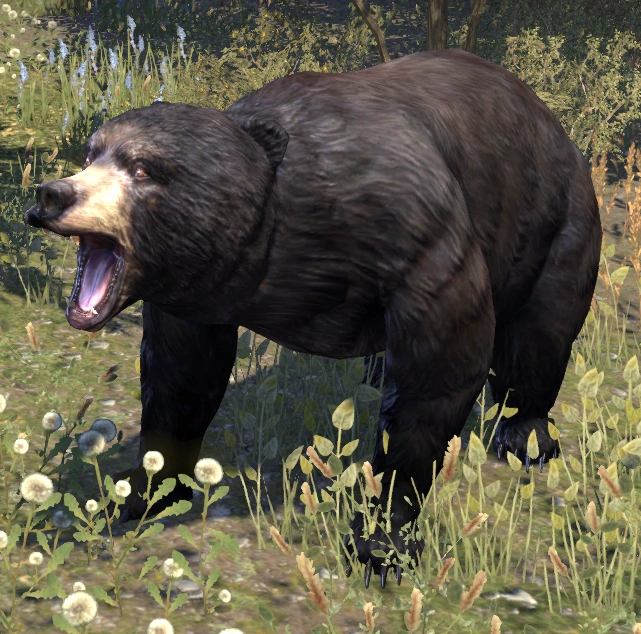
\includegraphics[scale=0.5]{bear.png}
\end{figure}

\subsubsection{Boars}
Boars are small, relatively slow animals with dangerous tusks. They are the only hostile animal that is not found in ruins or caves. Boars are only found outside, in Plains, Swamps, Forest, and Rainforest regions. All boars have 20\% frost resistance and a 10\% chance of infecting targets with the disease Chanthrax Blight. They attack by charging and attempting to gore targets with their tusks. Boars have a speed of 20 feet.\\

\begin{tabular}{|c|c|c|c|c|c|}
\hline
Name & Level & Health & Attack & Damage & Soul\\ \hline
Boar & 5--7 & 100 & 40\%--50\% & 24 physical, melee & Lesser\\ \hline
\end{tabular}\\

\begin{figure}[h]
	\centering
	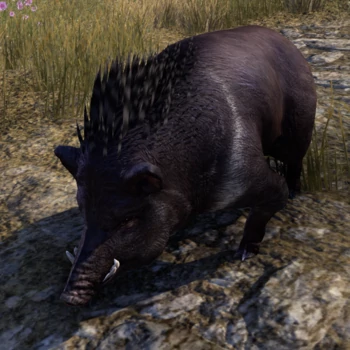
\includegraphics[scale=1]{boar.png}
\end{figure}

\subsubsection{Deer}
Deer are non-aggressive animals that even when attacked will prefer to flee. Deer are never found in caves and ruins. Deer are found starting at level 1 in any type of terrain. Deer are quite fast (speed 60 feet), so if you wish to hunt deer, you need to use ranged attacks, sneak up on them under the cover of night or magic, or have a very high running speed yourself. The male bucks can be identified by their antlers, and also have a different-colored hide than the female does. All deer have a 10\% chance of being infected with the disease Dampworm.\\

\begin{tabular}{|c|c|c|c|c|c|}
\hline
Name & Level & Health & Attack & Damage & Soul\\ \hline
Buck & 1 & 23 & 30\% & 10 physical, melee & Petty\\ \hline
Doe & 1 & 12 & 20\% & 4 physical, melee & Petty\\ \hline
\end{tabular}\\

\begin{figure}[h]
	\centering
	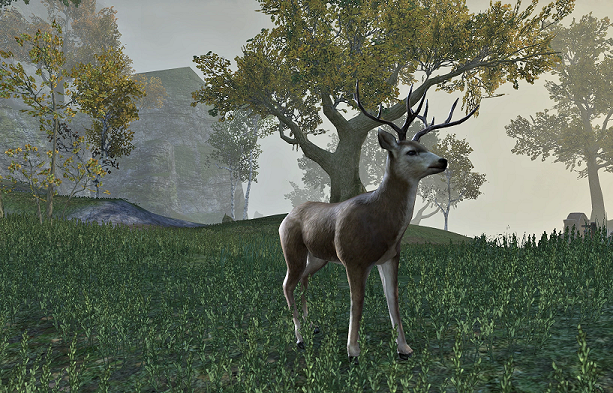
\includegraphics[scale=0.75]{deer.png}
\end{figure}

\subsubsection{Dogs}
Dogs are domesticated animals (in appearance they are nearly identical to wolves); whether or not they are friendly depends upon who owns them. Dogs primarily attack by biting. Dogs have a 10\% chance of being infected with Witbane. Dogs have a speed of 30 feet.

\begin{tabular}{|c|c|c|c|c|c|}
\hline
Name & Level & Health & Attack & Damage & Soul\\ \hline
Dog & 1 & 20 & 35\% & 8 physical, melee & Petty\\ \hline
\end{tabular}\\

\begin{figure}[h]
	\centering
	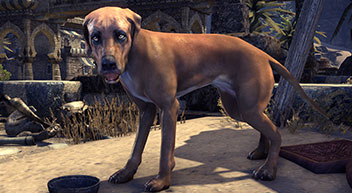
\includegraphics[scale=1]{dog.png}
\end{figure}

\subsubsection{Mountain Lions}
Mountain lions are rapid and vicious predators. They sometimes appear in caves and ruins. They are also randomly found outside in Farm, Plain, Rainforest, Highlands, and Mountain regions. They may be found starting at level 10 as boss-level creatures. Mountain lions are very fast (speed of 50 feet). They all have 20\% frost resistance and a 10\% chance of being infected with Wither.\\

\begin{tabular}{|c|c|c|c|c|c|}
\hline
Name & Level & Health & Attack & Damage & Soul\\ \hline
Mountain Lion & 10 & 160 & 55\% & 32 physical, melee & Common\\ \hline
\end{tabular}\\

\begin{figure}[h]
	\centering
	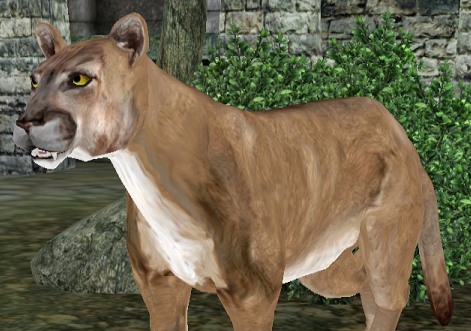
\includegraphics[scale=1]{mountainlion.png}
\end{figure}

\subsubsection{Mud Crabs}
Mud Crabs are weak nuisance creatures found everywhere near water. Although larger than many crabs on Nirn, they are smaller than most other animals encountered in Tamriel. Outside, they are found in swampy areas, along coastlines, and in shallow water. In caves and ruins, they are found in "Wet Lairs," just about any area with water. Mud Crabs are also very common in sewers. Mud Crabs attack with their claws. They have a 15\% chance of being infected with Swamp Fever. Mud crabs have a speed of 5 feet.

\begin{tabular}{|c|c|c|c|c|c|}
\hline
Name & Level & Health & Attack & Damage & Soul\\ \hline
Mud Crab & 1 & 10 & 20\% & 8 physical, melee & Petty\\ \hline
\end{tabular}\\

\begin{figure}[h]
	\centering
	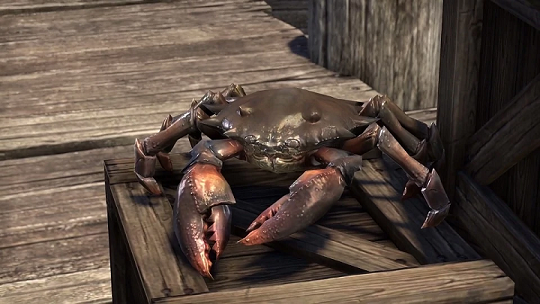
\includegraphics[scale=0.75]{mudcrab.png}
\end{figure}

\subsubsection{Rats}
Rats are the second type of weak nuisance creature that can be found nearly everywhere. As with Mud Crabs, they are oversized compared to many rats on earth, but are still relatively small compared to Tamriel animals. Outside, they are found in Farm, Valley, Forest, and Rainforest terrains. In caves and ruins, they are found in "Dry Lairs." Rats are also very common in sewers and in goblin lairs (where they are farmed for their rat meat). Rats tend to jump up and bite; their hyperactive bounciness can be much more annoying than the minor damage that they do. Rats have a speed of 10 feet and come with a 25\% chance of being infected with one of seven diseases: Blood Lung, Bone Break Fever, Brain Rot, Feeble Limb, Red Rage, Shakes or Witless Pox.\\

\begin{tabular}{|c|c|c|c|c|c|}
\hline
Name & Level & Health & Attack & Damage & Soul\\ \hline
Rat & 1 & 4 & 35\% & 2 physical, melee & Petty\\ \hline
\end{tabular}\\

\begin{figure}[h]
	\centering
	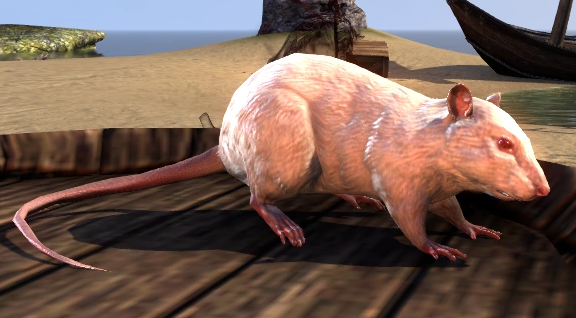
\includegraphics[scale=0.5]{rat.png}
\end{figure}

\subsubsection{Sheep}
Sheep are the least aggressive animals in Tamriel; many do not even have the ability to fight back if attacked. Sheep are all found in farms and sheepfolds. Sheep have a speed of 10 feet and a 10\% chance of being infected with Droops. Attacking sheep is generally illegal because sheep are usually the property of a farmer or shepherd. In the unlikely condition you find yourself assaulted by a sheep, you may have some explaining to do.

\begin{tabular}{|c|c|c|c|c|c|}
\hline
Name & Level & Health & Attack & Damage & Soul\\ \hline
Rat & 1 & 13 & 20\% & 3 physical, melee & Petty\\ \hline
\end{tabular}\\

\begin{figure}[h]
	\centering
	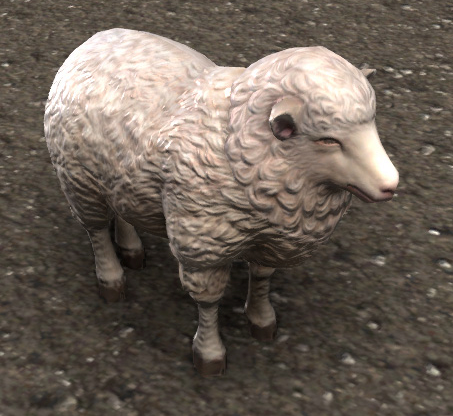
\includegraphics[scale=0.5]{sheep.png}
\end{figure}

\subsubsection{Slaughterfish}

\begin{figure}[h]
	\centering
	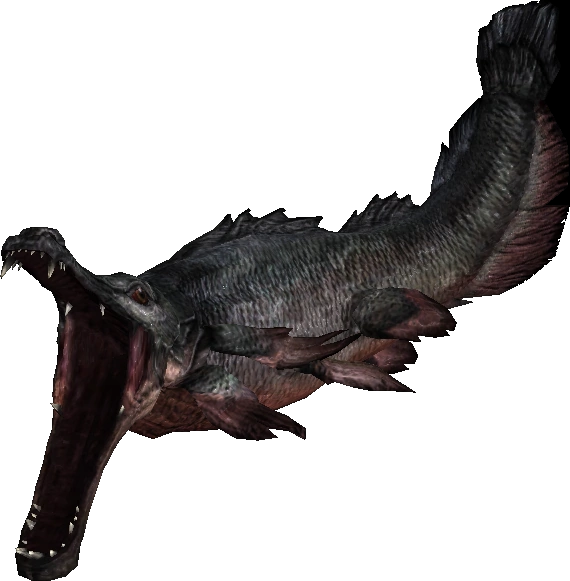
\includegraphics[scale=0.3]{slaughterfish.png}
\end{figure}

Slaughterfish are a predatory species of fish with long, razor-sharp teeth. They swim very quickly (swim speed 30 feet) and can be found in virtually all deep waters across Tamriel. They might also be found in submerged ruins or caves. On land, their speed is 2 feet and they are completely unable to attack. They are highly hazardous for characters not suited for aquatic conditions. Slaughterfish have a 25\% vulnerability to shock damage and a 10\% chance of being infected with Greenspore. They can see well in murky water. Some larger varieties are known to exist.\\

\begin{tabular}{|c|c|c|c|c|c|}
\hline
Name & Level & Health & Attack & Damage & Soul\\ \hline
Slaughterfish & 1 & 13 & 40\% & 15 physical, melee & Petty\\ \hline
Giant Slaughterfish & 10 & 130 & 65\% & 30 physical, melee & Common\\ \hline
\end{tabular}\\

\subsubsection{Wolves}
Wolves are fast and tenacious opponents. They come in two varieties: normal and timber. Both types of wolves are common throughout Tamriel: they can be found outside in all types of terrain except Swamp and Rainforest. They are also found in caves and mines, and they are common in vampire lairs. Wolves generally attack by biting; their speed (45 feet) can make them more difficult to kill. Timber wolves are generally larger and do more damage. All wolves have 20\% frost resistance and a 10\% chance of being infected with Helljoint. While they do not do much damage on their own, they tend to travel in organized packs.

\begin{tabular}{|c|c|c|c|c|c|}
\hline
Name & Level & Health & Attack & Damage & Soul\\ \hline
Wolf & 1 & 20 & 35\% & 10 physical, melee & Petty\\ \hline
Timber Wolf & 6 & 60 & 45\% & 20 physical, melee & Lesser\\ \hline
\end{tabular}\\

\begin{figure}[h]
	\centering
	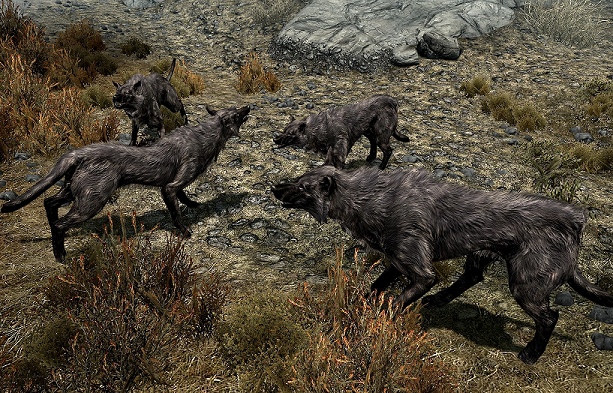
\includegraphics[scale=0.8]{wolves.png}
\end{figure}

\subsection{Daedra}
Daedra are creatures from the planes of Oblivion. The word comes from ancient elven languages and means "not our ancestors," as opposed to "aedra" which means "our ancestors." Strictly speaking, the word "daedra" is the plural form of "daedroth," but in common usage, "daedra" is typically the singular. This is further confused by the existence of a particular type of daedra known only as a daedroth, of which the plural form is typically written "daedroth" or "daedroths." Daedra often have magical powers and resistances. Most commonly, they are highly resistant to fire and somewhat weak to shock. Conjurers love to rely on them in battle.

Most creatures of this category can be summoned by the use of Conjuration magic. When slain, daedra might drop daedric items, loot stolen from mortals they've come across, or even body parts that are of great alchemical use. Note that this list is only a fraction of the varieties of daedra that exist in the Elder Scrolls.

For humanoid daedra (dremora), use the rules for making humanoid NPCs. There are special stat blocks for them which may be found here: \url{http://en.uesp.net/wiki/Oblivion:Dremora}.

\subsubsection{Atronachs}
Atronachs are beings of pure elemental power. They commonly come in three varieties: flame, frost and storm. Each variety is stronger than the last. There are rumored to be more kinds, but you would have a hard time finding them. All atronachs have a variety of elemental attacks, but each has unique features. All atronachs are immune to silence.

\begin{figure}[h]
	\begin{subfigure}{0.3\textwidth}
		\centering
		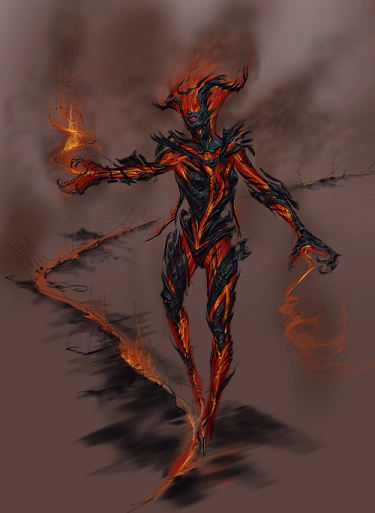
\includegraphics[scale=0.5]{flameatronach.png}
	\end{subfigure}
	\begin{subfigure}{0.3\textwidth}
		\centering
		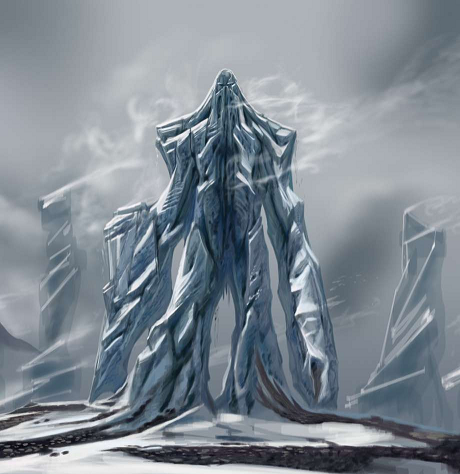
\includegraphics[scale=0.4]{frostatronach.png}
	\end{subfigure}
	\begin{subfigure}{0.3\textwidth}
		\centering
		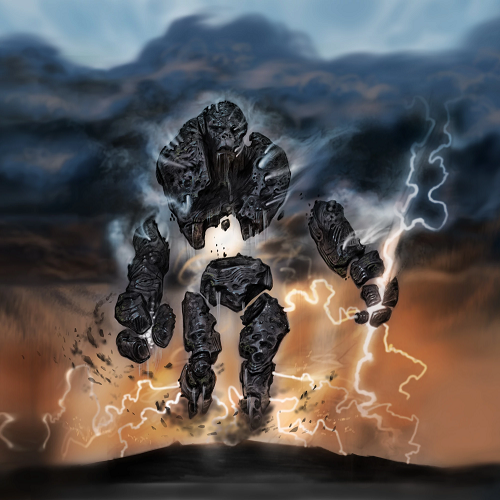
\includegraphics[scale=0.45]{stormatronach.png}
	\end{subfigure}
\end{figure}

Flame Atronachs are the weakest of the three elemental atronachs. They appear as a semi-humanoid, female form with blackened armor (that cannot be looted) and are surrounded by a veil of flames. Their primary attack is using Fire Damage spells. This atronach has one major weakness that you can turn to your advantage: the attack pattern is painfully obvious at distanced range. They prefer to stay at a distance, in fact. If at close quarters, they will flail around wildly, hitting you with whatever they possibly can. Flame atronachs are completely immune to fire and poison damage, and they reflect 15\% physical damage. However, they have a 50\% vulnerability to frost. They do not appear to be harmed by water, but they cannot swim and will move very slowly if submerged. Their land speed is 30 feet.

Frost Atronachs are the intermediate-difficulty elemental atronachs. They appear as a giant, humanoid figure composed entirely of ice. Their primary attack is using Frost Damage spells (they have both touch and targeted versions). They also have a strong melee attack. Unlike Flame Atronachs, Frost Atronachs will actively pursue the player once detected. They are able to heal themselves for 50 points as an action, so rapid attacks are recommended. They are completely immune to frost and poison damage and reflect 15\% physical damage, but they have a 50\% vulnerability to fire. Their speed is 30 feet.

Storm Atronachs are Daedra of elemental shock, and are the strongest elemental atronachs that are encountered in Oblivion. They appear as a cluster of rocks quickly revolving around an unseen center of mass. Their primary attack is using Shock Damage spells (they have both touch and ranged versions). They also have a strong melee attack. They are completely immune to shock and poison damage, reflect 15\% physical damage and cannot be paralyzed. Unlike the other two atronach varieties, storm atronachs have no vulnerability. They are very tough foes, and only masters of Conjuration can summon them.

\begin{tabular}{|c|c|c|c|p{0.15\textwidth}|c|}
\hline
Name & Level & Health & Attack & Damage & Soul\\ \hline
Flame Atronach & 9 & 150 & 50\% & 13 fire, melee, 5 physical, melee OR 8 fire, ranged (100 ft) & Common\\ \hline
Frost Atronach & 15 & 280 & 75\% & 40 frost, melee or physical OR 20 frost, ranged & Greater\\ \hline
Storm Atronach & 19 & 350 & 90\% & 50 shock, ranged, 20 points shock, melee or 26 points physical, melee & Lesser\\ \hline
\end{tabular}\\

\subsubsection{Clannfears}

\begin{figure}[h]
	\centering
	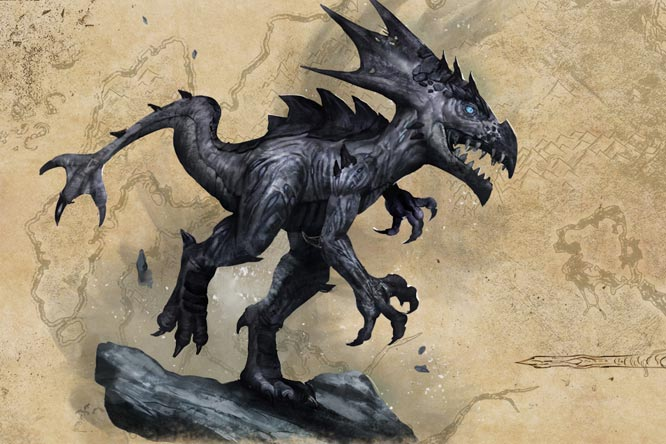
\includegraphics[scale=0.5]{clannfear.png}
\end{figure}

Clannfears are dinosaur-like Daedra that resemble a lizard with a large, bony crest on their head and a sharp beak and talons. They may represent common, wild animals in Oblivion. The Clannfear Runt is a weaker version of the Clannfear that is encountered at lower levels. Due to their great speed (45 feet) and considerable strength, they are fearsome opponents, especially at lower levels. All clannfears rely upon melee attacks using their heads, beaks, and/or claws. Their tough skin gives them 33\% resistance to fire and 20\% physical damage reflection, but they have a 20\% vulnerability to shock damage.\\

\begin{tabular}{|c|c|c|c|c|c|}
\hline
Name & Level & Health & Attack & Damage & Soul\\ \hline
Clannfear Runt & 5 & 75 & 45\% & 15 physical, melee & Lesser\\ \hline
Clannfear & 13 & 180 & 65\% & 36 physical, melee & Common\\ \hline
\end{tabular}\\

\subsubsection{Daedroths}

\begin{figure}[h]
	\centering
	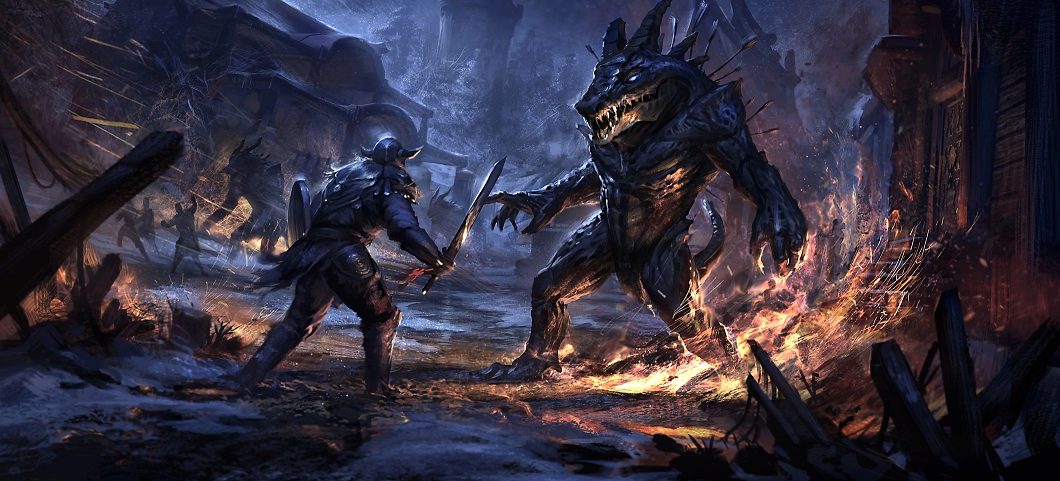
\includegraphics[scale=0.6]{daedroth.png}
\end{figure}

Daedroths are another type of beast-like Daedra believed to be common as wild animals in Oblivion. (When talking of this specific creature, Daedroths is an acceptable plural form of Daedroth). They resemble large crocodiles who walk upright. Daedroths will attack with their huge, clawed hands in melee. At range, they will breathe fire. They are 33\% resistant to fire, but they are also 20\% vulnerable to shock. A daedroth's speed is 30 feet. Daedroths can also cast a 25\% shield on themselves for 7 rounds as an action.

\begin{tabular}{|c|c|c|c|p{0.15\textwidth}|c|}
\hline
Name & Level & Health & Attack & Damage & Soul\\ \hline
Daedroth & 16 & 280 & 65\% & 20 fire, ranged (60 ft, 5-ft radius) OR 40 physical, melee & Greater\\ \hline
\end{tabular}\\

\subsubsection{Scamps}
Scamps are the weakest Daedra encountered in Oblivion (especially the smaller, weaker version, Stunted Scamps). Stunted Scamps primarily use a fire spell, even if you come close to them, but will occasionally use a melee attack. Regular Scamps generally cast their Scamp Reflection greater power (10\% chance to reflect spells) on themselves before starting to fight. If you are close to them, Regular Scamps primarily use melee attacks but otherwise use their fireball spell. All scamps have a 33\% resistance to fire and a 20\% weakness to shock. Normal-sized scamps have a speed of 30 feet. Stunted scamps have a speed of 20 feet.

\begin{figure}[h]
	\centering
	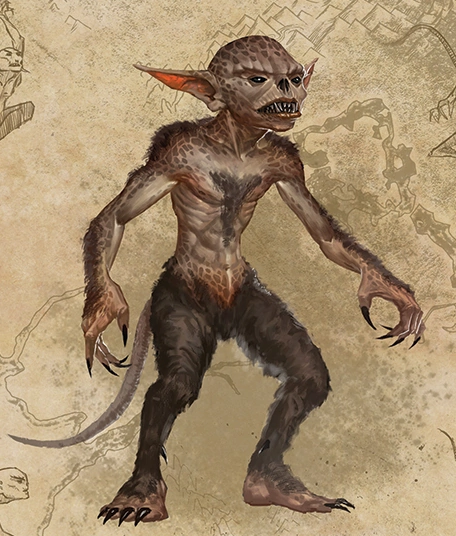
\includegraphics[scale=0.75]{scamp.png}
\end{figure}

\begin{tabular}{|c|c|c|c|p{0.15\textwidth}|c|}
\hline
Name & Level & Health & Attack & Damage & Soul\\ \hline
Stunted Scamp & 1 & 40 & 35\% & 6 fire, ranged (60 ft) OR 10 physical, melee & Petty\\ \hline
Scamp & 7 & 80 & 50\% & 10 fire, ranged (60 ft) OR 15 physical, melee & Lesser\\ \hline
\end{tabular}\\

When summoned, a scamp's health is equal to $16*PlayerLevel+1$, up to a maximum of 80.

\subsubsection{Spider Daedra}
Spider Daedra are relatively powerful Daedra, encountered starting at level 18. They look like giant spiders with human female torsos. Spider Daedra will always summon Spiderlings, which are identical in appearance to Spider Daedra except smaller. In combat, Spider Daedra rely upon their Spiderlings to keep you occupied, while they keep their distance and cast Shock Damage spells at you. The Spiderlings will run up and spit at you; the spit's paralysis effect is particularly dangerous. It is best to ignore the Spiderling and focus on killing the Spider Daedra; if the Spiderling is killed, another will just be immediately summoned. You can use Dispel on the Spider Daedra to easily get rid of the Spiderlings, which will cause the mother to drop everything and summon another, giving you lots of free hits. If forced into close combat, Spider Daedra will also use their melee attack which is enhanced by Poison Spit; unlike the Spiderling, the spit does not cause paralysis, but instead damages your health, speed, and agility. Spider Daedra also have the ability to heal themselves for 40 health as an action. Spider Daedra and their Spiderlings are immune to paralysis and have a 33\% resistance to fire, a 20\% vulnerability to shock and a 30\% vulnerability to frost. Spider Daedra have a speed of 30 feet, and Spiderlings have a speed of 20 feet.

\begin{tabular}{|c|c|c|c|p{0.15\textwidth}|c|}
\hline
Name & Level & Health & Attack & Damage & Soul\\ \hline
Spider Daedra & 18 & 300 & 85\% & 20 shock, ranged (100 ft), 40 poison, melee (drains 10 Agility and Speed for 2 rds) OR 16 physical, melee & Greater\\ \hline
Spiderling & N/A & 75 & 75\% & 10 poison, melee (paralyze 1 rd) OR 8 physical, melee & None\\ \hline
\end{tabular}\\

\begin{figure}[h]
	\centering
	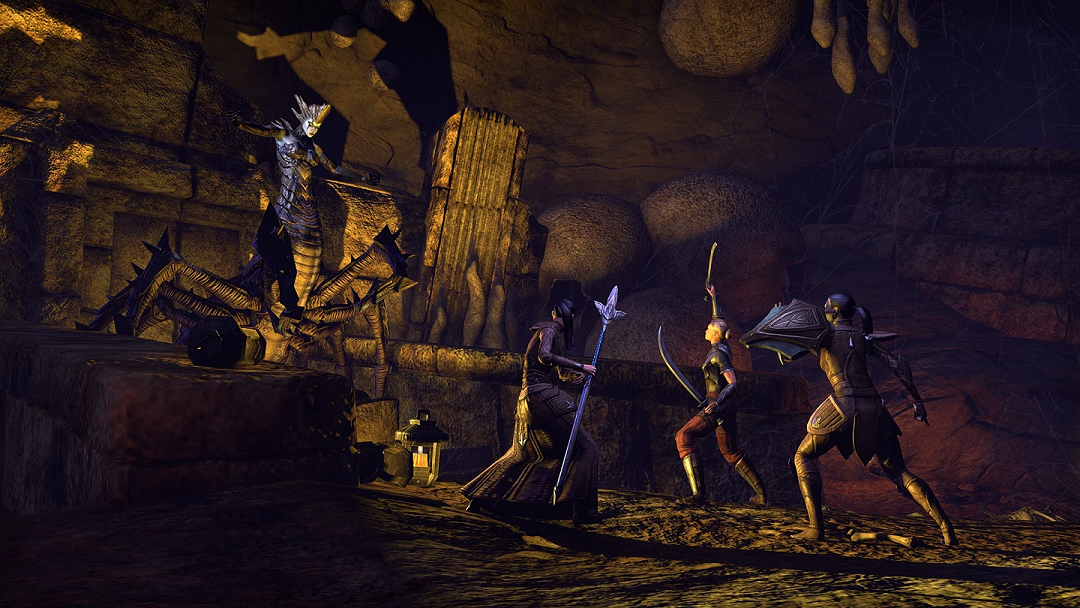
\includegraphics[scale=0.75]{spiderdaedra.png}
\end{figure}

\subsubsection{Xivilai}

Xivilai are highly intelligent, humanoid daedra that can be encountered at higher levels. Though highly similar to dremora, they have a few notable differences:

\begin{itemize}
	\item Their social structure does not have the caste system that dremora society does.
	\item They do not count as humanoids for some reason and do not require black soul gems for soul trapping.
	\item They do not appear in armor and rely primarily on spellcasting, though they typically have a weapon as well (two-handed weapon of daedric or ebony quality).
\end{itemize}

\begin{figure}[h]
	\centering
	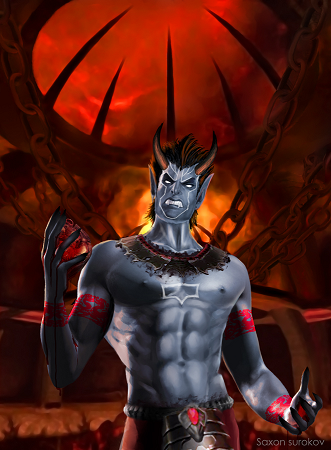
\includegraphics[scale=1]{xivilai.png}
\end{figure}

Xivilai know fire, frost and shock spells. They cannot regenerate magicka and instead rely on their generous spell absorption (50\%) and max magicka (400). They can summon clannfears and will typically do so at the start of a battle. They also know a damage reduction spell. They all have 33\% fire resistance and 20\% shock vulnerability. They have a speed of 30 feet. Xivilai known the following spells:

\begin{itemize}
	\item Heat Blast (70 fire damage, range 180 ft, 258 magicka)
	\item Lightning Surge (80 shock damage on touch, 212 magicka)
	\item Lightning Grasp (45 shock damage on touch, 101 magicka)
	\item Summon Clannfear (Clannfear for 7 rds, 340 magicka)
	\item Dispel Other (Dispel Journeyman effects, range 180 feet, 41 magicka)
	\item Guard (30\% physical resistance on self for 5 rds, 104 magicka)
\end{itemize}

\begin{tabular}{|c|c|c|c|p{0.15\textwidth}|c|}
\hline
Name & Level & Health & Attack & Damage & Soul\\ \hline
Xivilai & 18 & 240 & 85\% & 30 physical, melee OR spell list & Grand\\ \hline
\end{tabular}\\

\subsection{Goblins}
Goblins are the most common type of humanoid monster, and are treated differently from other monsters in Oblivion. Goblins tend to live in groups in underground caves, abandoned mines and ancient ruins, the entrances of which are often guarded and decorated with at least one stake with human skulls on it driven into the ground. They are the most sophisticated creatures in the game, with many goblins having a rank and job in the group.

\subsubsection{Goblin Culture}

About half of the goblins belong to one of eight tribes. Tribes represent the high point of goblin culture in the game and follow several rules. In the case of seven of the eight tribes, each tribe has its own home base cave, shaman, war chief and tribal totem staff. All members of a tribe have a tribal symbol visible on their upper right arm. Members of any tribe hate members of all other tribes. However, they will sometimes tolerate goblins who do not belong to any tribes.

The shaman functions as a spiritual leader who guards the tribe's sacred totem staff. The totem is a magic staff that belongs to the tribe (although the totems all look identical, each tribe recognizes its own totem). The shaman rarely leaves the cave and does not respawn. If one is killed, the tribe is without a spiritual leader and will no longer go to war over their totem. Likewise, the goblins will become passive towards outsiders, and allow them to traverse their lairs without protest. However, they will still attack them in self-defense. Each tribe also has a war chief as their military leader. Totems are kept in a specially designated place in the deepest part of the cave. Captured totems are also kept in a designated place about two thirds of the way into the cave.

The Bitterfish Tribe is the main exception to goblin tribal culture. It does not have a war chief, totem, or tribal symbol in the game. They do, however, seem to compensate for this by having multiple shamans (but unlike most of the other tribes, killing these shamans will not affect the behavior of the other tribe members). Another anomaly is that a Breton named Goblin Jim acts as the White Skin tribe's shaman. Like the Bitterfish tribe, the White Skins' behavior is unaffected by whether or not their de facto shaman is still alive.

\begin{figure}[h]
	\centering
	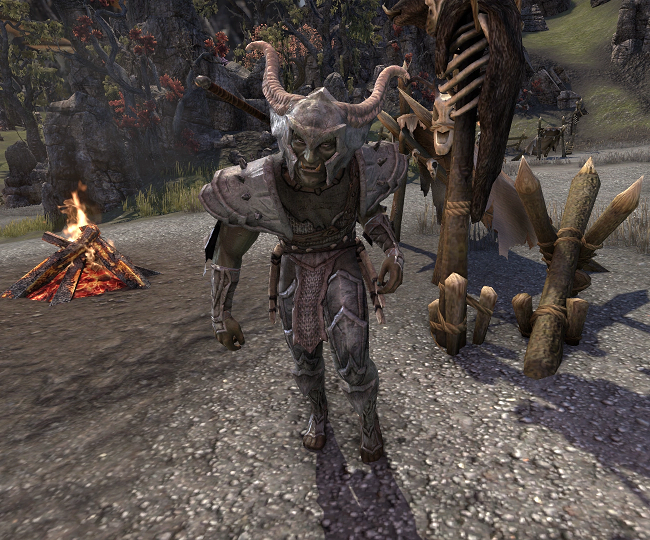
\includegraphics[scale=0.75]{goblin.png}
\end{figure}

Goblins in each tribe will be one of the following archetypes and use the corresponding stats. Loot drops may vary by tribe, but in general they should include weapons, shields, poisons, lockpicks and meager amounts of gold. They may also have other items looted from people who trespassed on their lands or whom they attacked for other reasons. All goblins have a speed of 30 feet.

\begin{tabular}{p{0.15\textwidth}|p{0.12\textwidth}|p{0.15\textwidth}|p{0.15\textwidth}|p{0.13\textwidth}|p{0.15\textwidth}}
Name & Level & Health & Attacks & Soul & Other\\ \hline
Goblin & 1 & 15 & Iron weapon (30\%), Unarmed (30\%, 3 damage) & Petty & ...\\ \hline
Goblin Archer & 1 & 15 & Iron or Steel Bow (30\%), Iron weapon (30\%), Unarmed (30\%, 3 damage) & Petty & ...\\ \hline
Goblin Skirmisher & 6 & 75 & Iron weapon (45\%), Unarmed (45\%, 3 damage) & Lesser & May have a leather or steel shield.\\ \hline
Goblin Skirmisher Archer & 6 & 75 & Iron or Steel Bow (45\%), Iron weapon (45\%), Unarmed (45\%, 3 damage) & Lesser & May have a leather or steel shield.\\
\end{tabular}


\begin{tabular}{p{0.15\textwidth}|p{0.12\textwidth}|p{0.15\textwidth}|p{0.15\textwidth}|p{0.13\textwidth}|p{0.15\textwidth}}
Name & Level & Health & Attacks & Soul & Other\\ \hline
Goblin Berserker & 10 & 170 & Steel or Dwarven weapon (60\%), Unarmed (60\%, 4 damage) & Lesser & May have a random shield up to Dwemer quality.\\ \hline
Goblin Berserker & 10 & 170 & Iron-Elven Bow (60\%), Steel or Dwarven weapon (60\%), Unarmed (60\%, 4 damage) & Lesser & Bow may be enchanted.\\ \hline
Goblin Shaman & 15 & 11*(LV-5) & Leveled weapon (70\%), Unarmed (70\%, 12 damage), spell list & Greater & 30\% spell absorption. May carry a staff.\\ \hline
Goblin Warlord & 18 & 30*LV & Weapon (85\%), Unarmed (85\%, 20 damage) & Grand & Weapon up to Elven quality. Has 25\% magic resistance May have shield up to Elven quality.\\ \hline
Goblin Warlord Archer & 18 & 30*LV & Bow (85\%) Weapon (85\%), Unarmed (85\%, 20 damage) & Grand & Weapon up to Elven quality. Has 25\% magic resistance.\\
\end{tabular}

Goblin shamans can cast spells from the following list. They have a spell range of 150 ft, a max magicka of 300 and a regeneration rate of 12\%.\\
\begin{itemize}
	\item Lightning Bolt (110 magicka): 35 shock damage at range, 120 ft
	\item Frost Touch (45 magicka): 25 frost damage on touch
	\item Paralyze (142 magicka): paralysis 1 rd on touch
	\item Summon Headless Zombie (140 magicka): Headless zombie for 4 rounds
	\item Flame Shield (power): 30\% fire shield on self for 1 minute
	\item Heal Greater Wounds (92 magicka): Restore 40 health on self
\end{itemize}

\subsection{Monsters}
Monsters (also known as mythical creatures) are creatures with various magical abilities, ranging from magical attacks to various magical resistances. There are very few features common to all of the monsters in the game of Oblivion. Each one has different resistances and different modes of attack. Monsters may drop rare alchemical ingredients or enchanted items. Listed levels are when they first start appearing; if a variable stat is shown, that means the monster may be found at higher levels.

\subsubsection{Imps}
Imps are small, winged humanoids who attack with a destruction spell of a randomly determined element. In the wilderness, Imps are found outdoors in all terrains except Farmlands and Plains. Along roads, however, they are only found in Valleys and Hills. Alchemists hunt them for their gall. Imps will attack at range with one of the following spells. They have a spell range of 100 feet. Don't worry about their max magicka. Imps have a flying speed of 30 feet.

\begin{itemize}
	\item Flare: 6 fire damage at range
	\item Snowball: 10 frost damage at range
	\item Spark: 10 shock damage at range
\end{itemize}

Imps have the following stats:

\begin{tabular}{|c|c|c|c|c|c|}
\hline
Name & Level & Health & Attack & Damage & Soul\\ \hline
Imp & 1--3 & 100 & 35\%--45\% & 6 physical, melee & Petty--Lesser\\ \hline
\end{tabular}\\

\begin{figure}
	\centering
	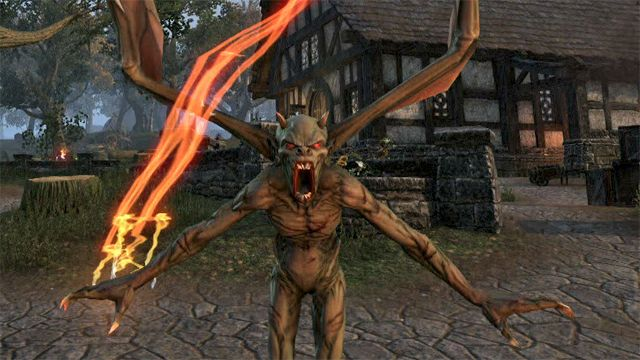
\includegraphics[scale=0.75]{imp.png}
\end{figure}

\subsubsection{Land Dreughs}

\begin{figure}[h]
	\centering
	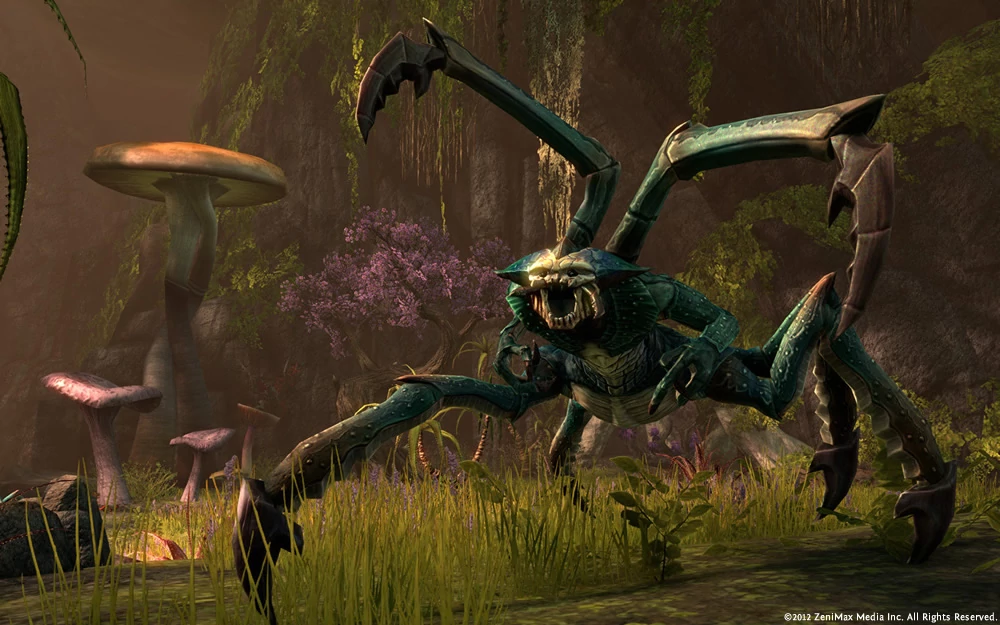
\includegraphics[scale=0.5]{dreugh.png}
\end{figure}

Dreughs are enormous crustacean creatures with scythe-like appendages and an innate capacity to discharge lethal electricity. Land Dreughs are actually a temporary metamorphosis of the "true" sea-dwelling Dreugh, which has appeared in earlier Elder Scrolls games. For one year of their life, dreughs undergo Karvinasim and emerge onto the land. In both their land-dwelling and aquatic forms, dreughs produce Dreugh Wax. Outdoors, Land Dreughs are only found in Swamp and Rainforest terrains. As mentioned in Brenus Astis' Journal and in conversation, the farmers call Land Dreughs "Billies". All dreughs have a 20\% resistance to magic and a 33\% resistance to non-magical weapons. Dreughs have a land speed of 40 feet and a swim speed of 50 feet.

\begin{tabular}{|c|c|c|c|p{0.15\textwidth}|c|}
\hline
Name & Level & Health & Attack & Damage & Soul\\ \hline
Land Dreugh & 17 & 320 & 75\% & 30 physical, melee OR 32 shock, melee & Greater\\ \hline
\end{tabular}\\

\subsubsection{Minotaurs}
Minotaurs are large, aggressive, and powerful humanoids with the head and legs of a bull, but the torso of a human. Outdoors, minotaurs are encountered in Hills and Forest Mountains terrains. They can attack with their powerful arms, but they are also quite fond of lowering their horns and charging. This attack is known to punch through armor and leave it broken, exposing unfortunate opponents to further attack. Less fortunate travelers may also come upon a larger variety of minotaurs known as minotaur lords. Minotaurs have a speed of 45 feet.

\begin{figure}[h]
	\centering
	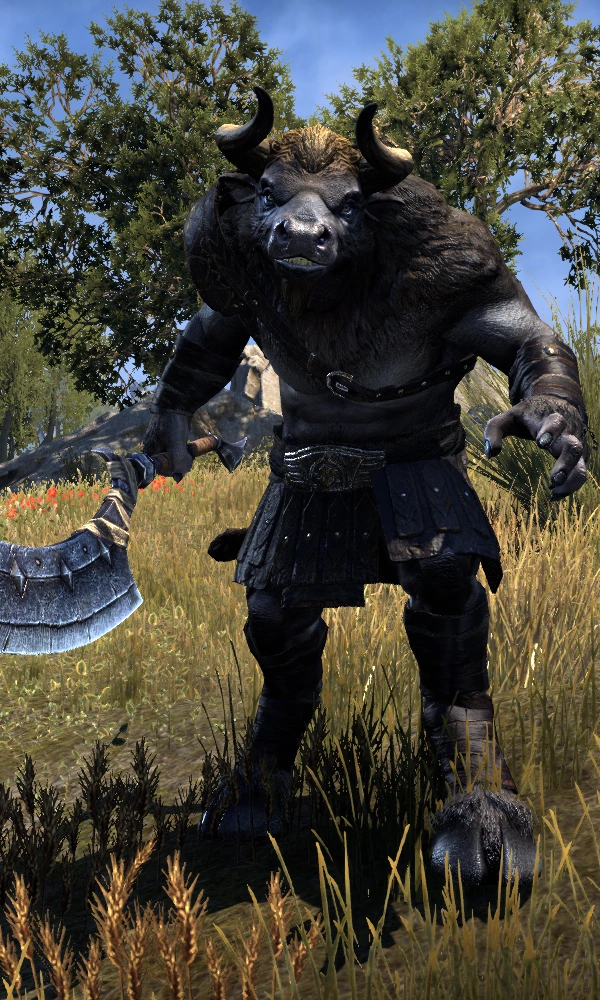
\includegraphics[scale=0.3]{minotaur.png}
\end{figure}

\begin{tabular}{|c|c|c|c|p{0.15\textwidth}|c|}
\hline
Name & Level & Health & Attack & Damage & Soul\\ \hline
Minotaur & 14 & 300 & 70\% & 30 physical, melee & Common\\ \hline
Minotaur Lord & 18 & 22*LV & 85\% & 40 physical, melee & Grand\\ \hline
\end{tabular}\\

\subsubsection{Ogres}
Ogres are huge, ugly, unarmed humanoids with pale blue skin and tremendous strength. Ogres are found outdoors in Hills, Highlands, Mountains, and Snowy Mountain terrains. They have a 25\% weakness to poisons of all types. Ogres have a speed of 35 feet.\\

\begin{tabular}{|c|c|c|c|p{0.15\textwidth}|c|}
\hline
Name & Level & Health & Attack & Damage & Soul\\ \hline
Ogre & 18 & 26*(LV-3) & 80\% & 30 physical, melee & Greater--Grand\\ \hline
\end{tabular}\\

\begin{figure}[h]
	\centering
	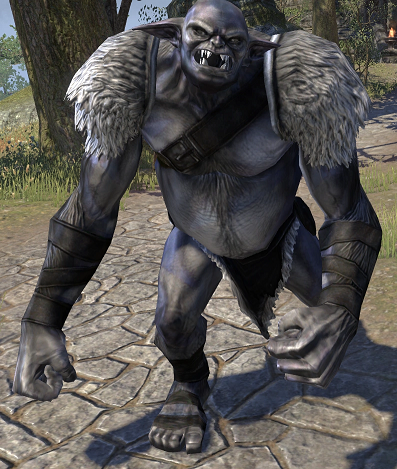
\includegraphics[scale=1]{ogre.png}
\end{figure}

\subsubsection{Spriggans}
Spriggans resemble a cross between a tree and human woman. They may summon a Black Bear once per day, and their variety of abilities make them very dangerous opponents. They are able to fully replenish their health three times a day. Outdoors, Spriggans are found along roads in Forest terrains, and in the wilderness in Swamp and Forest terrains. They emit quiet, giggling laughter when idle. All spriggans have a 30\% vulnerability to fire and a 30\% resistance to shock. They are immune to silence. Spriggans have a speed of 30 feet.

\begin{tabular}{|c|c|c|c|p{0.15\textwidth}|c|}
\hline
Name & Level & Health & Attack & Damage & Soul\\ \hline
Spriggan & 13 & 175 & 65\% & 20 physical, melee OR 20 magical, melee & Common\\ \hline
\end{tabular}\\

\begin{figure}[h]
	\centering
	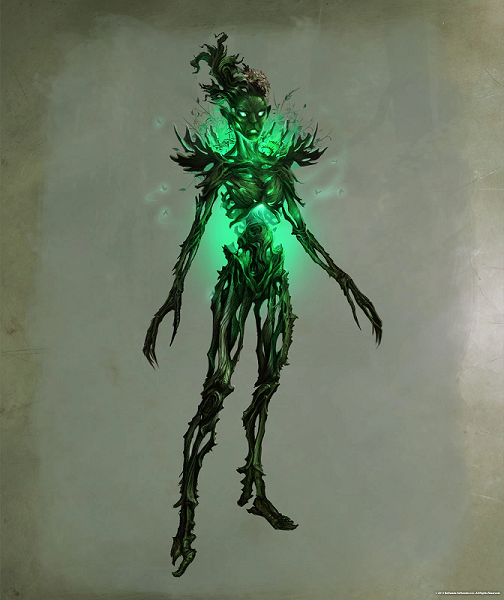
\includegraphics[scale=0.8]{spriggan.png}
\end{figure}

\subsubsection{Trolls}
Trolls resemble green apes with three eyes, and have a distinctive battle howl. They are extremely fast (speed of 50 feet), deal considerable damage and regenerate health, making them potentially dangerous opponents at all levels. Outdoors, Trolls are found in Forest and Rainforest terrains. All trolls are 50\% vulnerable to fire attacks and recover 10\% of their max health per round. Damage suffered from fire attacks can only recover at half this rate.

\begin{tabular}{|c|c|c|c|p{0.15\textwidth}|c|}
\hline
Name & Level & Health & Attack & Damage & Soul\\ \hline
Troll & 8 & 80 & 50\% & 12 physical, melee & Lesser\\ \hline
Swamp Troll & 12 & 13*LV & 60\% & 15 physical, melee & Common\\ \hline
\end{tabular}\\

\begin{figure}[h]
	\centering
	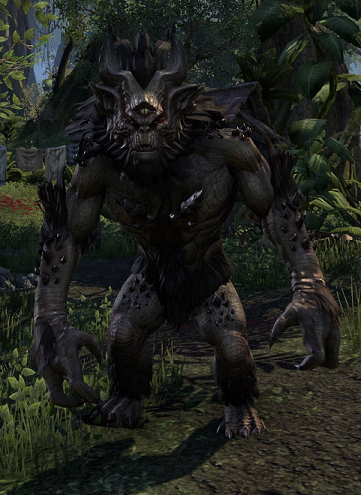
\includegraphics[scale=1]{troll.png}
\end{figure}

\subsubsection{Will-o-the-Wisps}
Will-o-the-Wisps are luminous beings seemingly composed of gas. They are immune to normal damage, silence, paralysis and poison, and have extremely dangerous magic. They are also very fast and have the ability to become nearly invisible. Outdoors, standard Will-o-the-Wisps are only found in Swamp terrains. When fighting Will-o-the-Wisps, the most important strategy is to focus on ranged attacks; do not let them come close enough to touch you, since both of their attacks are on-touch. Detect Life is extremely useful for seeing where they are located. Another option (if available) is to fight them in the water, since they leave a visible wake in the water, even when invisible. While in combat, they are always invisible except for the moment they attack. Preparing attacks may be useful. Will-o-the-Wisps have a speed of 40 ft.\\

\begin{tabular}{|c|c|c|c|p{0.15\textwidth}|c|}
\hline
Name & Level & Health & Attack & Damage & Soul\\ \hline
Will-o-the-Wisp & 11 & 220 & 65\% & Absorb 30 health and magicka on touch & Common\\ \hline
\end{tabular}\\

\begin{figure}[h]
	\centering
	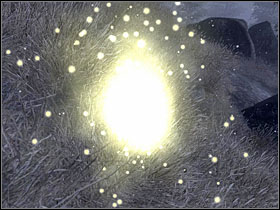
\includegraphics[scale=1]{willothewisp.png}
\end{figure}

\subsection{Undead}
Undead creatures consist of various forms of reanimated corpses and spirits. All undead are immune to poison, and resist frost to varying degrees. Undead cannot be drowned: they all have either Water Walking or Water Breathing as a permanent ability. They cannot be knocked unconscious. All undead can be affected by Turn Undead, but none can be affected by illusions. Most undead creatures can be summoned. Necromancers are very likely to rely on them in battle. Loot obtained from undead can be all manner of things, including weapons, magical items, armor, gold or even rare alchemical reagents.

\subsubsection{Ethereal}

\begin{figure}[h]
	\centering
	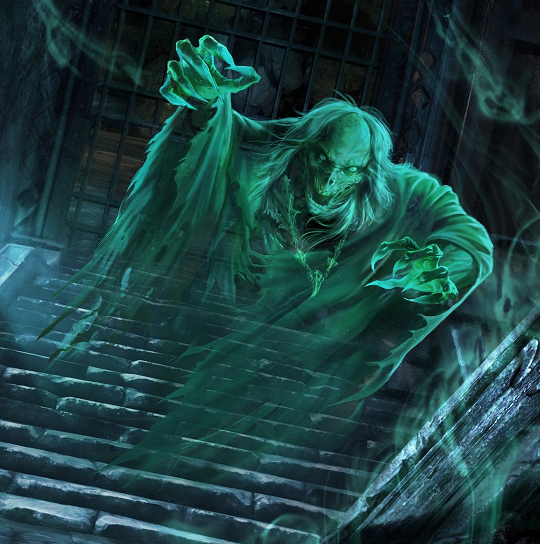
\includegraphics[scale=0.75]{wraith.png}
\end{figure}

Ethereal undead include all ghosts and wraiths. Ghosts rely upon magical attacks, in particular Frost Damage. Ancient Ghosts may turn invisible as a bonus action. As with Will-o-the-Wisps, preparing an action to strike when they are visible may be effective. Wraiths and all of their variants are often encountered throughout the darker parts of Cyrodiil. Wraiths are categorized into the weak Faded Wraiths, and the more powerful Wraiths. The higher level the wraith, the higher their health and the stronger their spells. All wraiths have a powerful curse that they can cast on you (effects vary with type of wraith) that is immune to silence. Most wraiths have several additional spells, in particular Frost Damage and Silence spells. In addition, about half of all wraiths carry a sword (shortsword or longsword of appropriate level). All ghosts and wraiths are immune to frost, poison and nonmagical weapons, and they have a fly speed of 40 feet. Their spell range is between 100 and 200 feet, depending on level. Use your judgement.

\begin{tabular}{|c|c|c|c|p{0.15\textwidth}|c|}
\hline
Name & Level & Health & Attack & Damage & Soul\\ \hline
Ghost & 6 & 18*(LV-1) & 50\% & 10 frost and stamina, melee or ranged & Lesser\\ \hline
Ancient Ghost & 11 & 170 & 65\% & 20 frost and stamina, melee or ranged & Common\\ \hline
Faded Wraith & 14 & 280 & 75\% & 45 frost, melee or ranged; 10 frost and silence 2 rds, ranged; 24 physical, melee & Common\\ \hline
Wraith & 18 & 400 & 85\% & 45 frost, melee or ranged; 10 frost and silence 2 rds, ranged; 24 physical, melee & Common\\ \hline
\end{tabular}\\

By succeeding on a ranged spell attack, Wraiths and Faded Wraiths can place a curse on targets. The Faded Wraith curse deals 10 frost damage, then an additional 6 per round for 5 rounds. It also lowers the target's Strength and Endurance by 20 points for 5 rounds. The Wraith's curse absorbs 12 health per round and lowers the target's Strength and Endurance by 30 points for 5 rounds. Wraiths are not to be trifled with. Both curses have a 25\% chance of leaving a lingering curse of 10 points to Strength and Endurance that can only be lifted at a Divine altar or by skilled Restoration mages.

\subsubsection{Liches}
Liches are powerful necromancers who have attained immortality through death and necromantic magic. They are incredibly powerful and generally only encountered at higher levels. They rely upon magical attacks, both from their staves and from their spells (which are generally randomly determined). They will also usually summon an undead underling. All liches have a 25\% vulnerability to fire, immunity to frost and poison, 25\% magic resistance and 25\% spell absorption. They have a fly speed of 40 feet. Some liches may also have 25\% spell reflection as well. Give them access to Expert and Master level spells, and do not worry about their magicka reserves; they are far too powerful to worry about that anymore.

\begin{figure}[h]
	\centering
	
\includegraphics[scale=1]{lich.png}
\end{figure}

\begin{tabular}{|c|c|c|c|p{0.15\textwidth}|c|}
\hline
Name & Level & Health & Attack & Damage & Soul\\ \hline
Lich & 18 & 360 & 90\% & 20 physical, melee OR spells & Grand\\ \hline
\end{tabular}\\

\subsubsection{Skeletons}
Skeletons are encountered at all levels. They rely upon weapons for attacking. Standard skeletons all come in both melee and archer varieties; the melee varieties are about twice as common. Skeletons all have a 75\% resistance to frost and complete immunity to poison and paralysis. They do not need to breathe underwater. Skeletons have a speed of 35 feet.

\begin{figure}[h]
	\centering
	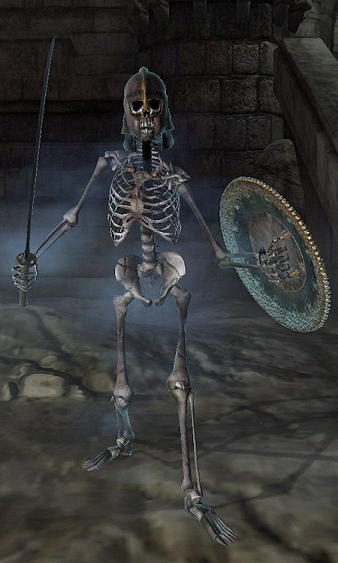
\includegraphics[scale=1]{skeleton.png}
\end{figure}

\begin{tabular}{|c|c|c|c|p{0.15\textwidth}|c|}
\hline
Name & Level & Health & Attack & Damage & Soul\\ \hline
Skeleton & 1 & 20 & 35\% & Iron/steel war axe or bow & Petty\\ \hline
Skeleton Guardian & 8 & 170 & 55\% & Steel-Elven mace or bow & Lesser\\ \hline
Skeleton Hero & 12 & 208 & 65\% & Steel-Elven mace or bow & Common\\ \hline
Skeleton Champion & 17 & 350 & 80\% & Steel-Glass claymore or bow & Greater\\ \hline
\end{tabular}\\

\subsubsection{Zombies}
Zombies are reanimated corpses. They have mottled, muddy green flesh, various deep and fatal-looking wounds, and they are often missing an arm. Zombies can be deceiving for players having not encountered one before, as they can run and give chase, and have a distinctive groaning voice when they detect prey. They rely upon unarmed melee attacks, which are made more dangerous by the many diseases that zombies can carry. Zombies have a 50\% vulnerability to fire and 30\% resistance to frost and magic. They are immune to poison. At higher levels, zombies have greater health, hit harder, and carry more diseases. Dread Zombies are able to regenerate 30 health per round.

\begin{figure}[h]
	\centering
	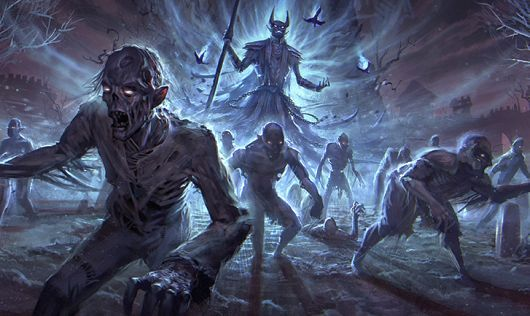
\includegraphics[scale=0.8]{zombiearmy.png}
\end{figure}

\begin{tabular}{|c|c|c|c|p{0.15\textwidth}|c|}
\hline
Name & Level & Health & Attack & Damage & Soul\\ \hline
Zombie & 4 & 80 & 45\% & 10 physical, melee & Lesser\\ \hline
Headless Zombie & 10 & 175 & 60\% & 27 physical, melee & Common\\ \hline
Dread Zombie & 16 & 340 & 75\% & 38 physical, melee & Greater\\ \hline
\end{tabular}\\

Zombies have a 25\% chance of carrying one of the following diseases: Ataxia, Brown Rot, Dampworm, Droops, Greenspore, Helljoint, Rockjoint, Rust Chancre or Witbane.

Headless Zombies have a 33\% chance of carrying one of the following diseases: Black-Heart Blight, Chanthrax Blight, Chills, Collywobbles, Rattles, Serpiginous Dementia, Swamp Fever, Wither or Yellow Tick.

All Dread Zombies carry Astral Vapors.

\chapter{Weapons and Armor}
The Player's Handbook contains brief descriptions of each weapon type and a base damage roll as well as a general description of armor types. The specific names and stats of the weapons and armors have been left out to give a sense of mystery to the variety of equipment in the world. Here, we will discuss the system for weapon and armor values as well as provide brief example lists.

\section{Weapons}
There are seven tiers of weapons: Iron, Steel, Dwemer, Elven, Glass, Ebony and Daedric. Regardless of which type of weapon you are considering, an increase in tier adds +1 to the weapon's damage formula. In case this is unclear, the weapons will be listed in tables below.

Seven is reduced from the number of weapon tiers present in the video games, as players are expected to max out at level 20. Levels beyond 20 are feasible according to the normal level up formula, but you may wish to create new weapons to support it.

\begin{tabular}{|p{0.2\textwidth}|p{0.2\textwidth}|p{0.2\textwidth}|p{0.2\textwidth}|}
\hline
Name & Base Damage & Level Range & Base Cost\\ \hline
Iron Dagger & 1d6 & 1--2 & 6\\ \hline
Steel Dagger & 1d6+1 & 3--5 & 20\\ \hline
Dwemer Dagger & 1d6+2 & 6--8 & 110\\ \hline
Elven Dagger & 1d6+3 & 9--11 & 260\\ \hline
Glass Dagger & 1d6+4 & 12--14 & 570\\ \hline
Ebony Dagger & 1d6+5 & 15--17 & 1250\\ \hline
Daedric Dagger & 1d6+6 & 18--20 & 2700\\ \hline
\end{tabular}

\begin{tabular}{|p{0.2\textwidth}|p{0.2\textwidth}|p{0.2\textwidth}|p{0.2\textwidth}|}
\hline
Name & Base Damage & Level Range & Base Cost\\ \hline
Iron Shortsword & 1d8 & 1--2 & 10\\ \hline
Steel Shortsword & 1d8+1 & 3--5 & 25\\ \hline
Dwemer Shortsword & 1d8+2 & 6--8 & 145\\ \hline
Elven Shortsword & 1d8+3 & 9--11 & 320\\ \hline
Glass Shortsword & 1d8+4 & 12--14 & 670\\ \hline
Ebony Shortsword & 1d8+5 & 15--17 & 1400\\ \hline
Daedric Shortsword & 1d8+6 & 18--20 & 2900\\ \hline
\end{tabular}

\begin{tabular}{|p{0.2\textwidth}|p{0.2\textwidth}|p{0.2\textwidth}|p{0.2\textwidth}|}
\hline
Name & Base Damage & Level Range & Base Cost\\ \hline
Iron Longsword & 1d10 & 1--2 & 20\\ \hline
Steel Longsword & 1d10+1 & 3--5 & 45\\ \hline
Dwemer Longsword & 1d10+2 & 6--8 & 200\\ \hline
Elven Longsword & 1d10+3 & 9--11 & 420\\ \hline
Glass Longsword & 1d10+4 & 12--14 & 840\\ \hline
Ebony Longsword & 1d10+5 & 15--17 & 1700\\ \hline
Daedric Longsword & 1d10+6 & 18--20 & 3100\\ \hline
\end{tabular}

\begin{tabular}{|p{0.2\textwidth}|p{0.2\textwidth}|p{0.2\textwidth}|p{0.2\textwidth}|}
\hline
Name & Base Damage & Level Range & Base Cost\\ \hline
Iron Claymore & 2d6 & 1--2 & 40\\ \hline
Steel Claymore & 2d6+1 & 3--5 & 80\\ \hline
Dwemer Claymore & 2d6+2 & 6--8 & 310\\ \hline
Elven Claymore & 2d6+3 & 9--11 & 600\\ \hline
Glass Claymore & 2d6+4 & 12--14 & 1150\\ \hline
Ebony Claymore & 2d6+5 & 15--17 & 2200\\ \hline
Daedric Claymore & 2d6+6 & 18--20 & 4000\\ \hline
\end{tabular}

\begin{tabular}{|p{0.2\textwidth}|p{0.2\textwidth}|p{0.2\textwidth}|p{0.2\textwidth}|}
\hline
Name & Base Damage & Level Range & Base Cost\\ \hline
Iron War Axe & 1d8 & 1--2 & 13\\ \hline
Steel War Axe & 1d8+1 & 3--5 & 35\\ \hline
Dwemer War Axe & 1d8+2 & 6--8 & 165\\ \hline
Elven War Axe & 1d8+3 & 9--11 & 345\\ \hline
Glass War Axe & 1d8+4 & 12--14 & 710\\ \hline
Ebony War Axe & 1d8+5 & 15--17 & 1450\\ \hline
Daedric War Axe & 1d8+6 & 18--20 & 3100\\ \hline
\end{tabular}

\chapter{Magical Effects}
All spells, scrolls, staves, potions, enchantments, powers and diseases make use of magical effects. Each one comes with a name, base cost and barter factor. The magical effects used in the ESTRPG are somewhat different than those in Oblivion. We have also created some new effects and incorporated effects from other Elder Scrolls titles into the system. You can of course create your own; try to remember the crafting formulas when you do. Also, be aware that magnitude has different meanings for different effects. In the descriptions, M is a variable for magnitude in points.

We begin with effects governed by Alteration:\\

\begin{tabular}{p{0.3\textwidth}|p{0.1\textwidth}|p{0.1\textwidth}|p{0.3\textwidth}}
Effect & Base Cost & Barter Factor & Description\\ \hline
Burden & 0.21 & 0 & Reduce the target's maximum encumbrance by M points.\\ \hline
Feather & 0.01 & 25 & Increase the target's maximum encumbrance by M points.\\ \hline
Fire Shield & 0.95 & 100 & Creates a fire shield (M\% physical \& fire resistance) around the target's body.\\
\end{tabular}

\begin{tabular}{p{0.3\textwidth}|p{0.1\textwidth}|p{0.1\textwidth}|p{0.3\textwidth}}
Effect & Base Cost & Barter Factor & Description\\ \hline
Frost Shield & 0.95 & 100 & Creates a frost shield (M\% physical and frost resistance) around the target's body.\\ \hline
Jump & 12 & 400 & Allows the target to jump M times farther and higher.\\ \hline
Levitation & 15.0 & 500 & Allows the target to fly M*30 feet per round. Illegal in the Empire.\\ \hline
Open & 4.3 & 0 & Opens a locked container or door.\\ \hline
Shield & 0.45 & 100 & Creates a magical shield that contributes to M\% of the level-appropriate longsword's expected damage value to the target's armor rating.\\ \hline
Shock Shield & 0.95 & 100 & Creates a shock shield ( M\% physical \& shock resistance) around the target's body.\\ \hline
Slow Fall & 11.0 & 300 & Slows falling speed M times, allowing the target to suffer less fall damage.\\ \hline
Swift Swim & 13.0 & 300 & Boosts the target's swim speed M times.\\ \hline
Water Breathing & 14.5 & 400 & Lets the target breathe underwater.\\ \hline
Water Walking & 13.0 & 400 & Lets the target walk on water.\\
\end{tabular}

\newpage
The following are Conjuration effects. Bound items weigh nothing and do not impose movement penalties. When attacking with a bound weapon, use the relevant weapon skill or Conjuration, whichever is higher.

\begin{tabular}{p{0.3\textwidth}|p{0.1\textwidth}|p{0.1\textwidth}|p{0.3\textwidth}}
Effect & Base Cost & Barter Factor & Description\\ \hline
Bound Armor & 8.0 & 75 & Equips the target with heavy or light armor of tier M. The armor appears Daedric.\\ \hline
Bound Weapon & 7.5 & 70 & Equips the target with a weapon of choice of tier M. Can summon shields of level M. Weapon appears Daedric and is magic.\\ \hline
Summon Clannfear & 75.56 & 0 & Summons a clannfear.\\ \hline
Summon Daedroth & 123.33 & 0 & Summons a daedroth.\\ \hline
Summon Dremora & 72.5 & 0 & Summons a dremora.\\ \hline
Summon Dremora Lord & 157.14 & 0 & Summons a Dremora Lord.\\ \hline
Summon Flame Atronach & 45.0 & 0 & Summons a flame atronach.\\ \hline
Summon Frost Atronach & 102.86 & 0 & Summons a frost atronach\\ \hline
Summon Ghost & 22.0 & 0 & Summons a ghost.\\ \hline
Summon Headless Zombie & 56.0 & 0 & Summons a headless zombie.\\ \hline
Summon Lich & 350.0 & 0 & Summons a lich.\\ \hline
Summon Scamp & 30.0 & 0 & Summons a scamp.\\ \hline
Summon Skeleton & 11.25 & 0 & Summons a skeleton.\\ \hline
Summon Skeleton Guardian & 32.5 & 0 & Summons a skeleton guardian.\\ \hline
Summon Skeleton Hero & 66.0 & 0 & Summons a skeleton hero.\\ \hline
Summon Skeleton Champion & 152.0 & 0 & Summons a skeleton champion.\\
\end{tabular}

\begin{tabular}{p{0.3\textwidth}|p{0.1\textwidth}|p{0.1\textwidth}|p{0.3\textwidth}}
Effect & Base Cost & Barter Factor & Description\\ \hline
Summon Spider Daedra & 195.0 & 0 & Summons a spider daedra.\\ \hline
Summon Storm Atronach & 125.0 & 0 & Summons a storm atronach.\\ \hline
Summon Faded Wraith & 87.5 & 0 & Summons a faded wraith.\\ \hline
Summon Wraith & 260.0 & 0 & Summons a wraith.\\ \hline
Summon Xivilai & 200.0 & 0 & Summons a xivilai.\\ \hline
Summon Zombie & 16.67 & 0 & Summons a zombie.\\ \hline
Turn Undead & 0.083 & 0 & Undead up to level M/4 are inflicted with fear and must use their movement to run away from the caster.\\
\end{tabular}

Destruction Effects

\begin{tabular}{p{0.3\textwidth}|p{0.1\textwidth}|p{0.1\textwidth}|p{0.3\textwidth}}
Effect & Base Cost & Barter Factor & Description\\ \hline
Damage Attribute & 100.0 & 0 & Damages the target's attribute by M*6 points per round until it is magically restored.\\ \hline
Damage Health & 12.0 & 0 & Damages target's health M points.\\ \hline
Damage Magicka & 2.45 & 0 & Damages target's magicka M points.\\ \hline
Damage Stamina & 4.4 & 0 & Damages target's stamina M points.\\ \hline
Disintegrate Armor & 6.2 & 0 & Damage armor, reducing its rating until it is repaired.\\ \hline
Disintegrate Weapon & 6.2 & 0 & Damage weapons, reducing their damage until they are repaired.\\
\end{tabular}

\begin{tabular}{p{0.3\textwidth}|p{0.1\textwidth}|p{0.1\textwidth}|p{0.3\textwidth}}
Effect & Base Cost & Barter Factor & Description\\ \hline
Drain Attribute & 0.7 & 0 & Lowers the target's attribute M points temporarily.\\ \hline
Drain Health & 0.9 & 0 & Temporarily lowers the target's max health M points.\\ \hline
Drain Magicka & 0.18 & 0 & Temporarily lowers the target's max magicka M points.\\ \hline
Drain Skill & 0.65 & 0 & Temporarily lowers the target's skill.\\ \hline
Drain Stamina & 0.18 & 0 & Temporarily lowers the target's max stamina.\\ \hline
Fire Damage & 7.5 & 0 & M points of fire damage on target.\\ \hline
Frost Damage & 7.4 & 0 & M points of frost damage on target.\\ \hline
Shock Damage & 7.8 & 0 & M points of shock damage on target.\\ \hline
Weakness to Disease & 0.12 & 0 & Reduces the target's resistance to disease M points.\\ \hline
Weakness to Fire & 0.1 & 0 & Reduces the target's resistance to fire M points.\\ \hline
Weakness to Frost & 0.1 & 0 & Reduces the target's resistance to frost M points.\\ \hline
Weakness to Magic & 0.25 & 0 & Reduces the target's resistance to magic M points.\\ \hline
Weakness to Normal Weapons & 0.25 & 0 & Reduces the target's resistance to normal weapons M points.\\
\end{tabular}

\begin{tabular}{p{0.3\textwidth}|p{0.1\textwidth}|p{0.1\textwidth}|p{0.3\textwidth}}
Effect & Base Cost & Barter Factor & Description\\ \hline
Weakness to Poison & 0.1 & 0 & Reduces the target's resistance to poison M points.\\ \hline
Weakness to Shock & 0.1 & 0 & Reduces the target's resistance to shock M points.
\end{tabular}

Illusion Effects

\begin{tabular}{p{0.3\textwidth}|p{0.1\textwidth}|p{0.1\textwidth}|p{0.3\textwidth}}
Effect & Base Cost & Barter Factor & Description\\ \hline
Calm & 0.47 & 0 & Targets up to level M/4 are calmed for the duration.\\ \hline
Chameleon & 0.63 & 65 & Blend into your surroundings, becoming lightly obscured for the duration.\\ \hline
Charm & 0.2 & 0 & Bonus die on Speechcraft checks.\\ \hline
Cacophony & 40.0 & 0 & Prevents a target from casting a spell.\\ \hline
Command Creature & 0.6 & 0 & Creatures up to level M/4 will fight for you for the duration. Effect wears off if you attack the target.\\ \hline
Command Humanoid & 0.75 & 0 & Humanoids up to level M/4 will fight for you for the duration. Effect wears off if you attack the target.\\ \hline
Fear & 0.49 & 0 & Inflicts fear on targets up to level M/4 for the duration.\\
\end{tabular}

\begin{tabular}{p{0.3\textwidth}|p{0.1\textwidth}|p{0.1\textwidth}|p{0.3\textwidth}}
Effect & Base Cost & Barter Factor & Description\\ \hline
Frenzy & 0.04 & 0 & Targets up to level M/4 are frenzied for the duration.\\ \hline
Invisibility & 40.0 & 0 & Makes the target invisible for the duration. Dissipates when any action is taken.\\ \hline
Light & 0.051 & 12.5 & The target gives off light in an M-foot radius.\\ \hline
Muffle & 25.0 & 30 & All other characters are deafened to you.\\ \hline
Night-Eye & 22.0 & 20 & The target can see in the dark.\\ \hline
Paralyze & 475 & 0 & Paralyzes the target for the duration.\\ \hline
Rally & 0.03 & 0 & Targets up to level M/4 are cured of calm, fear and frenzy.\\ \hline
Silence & 60.0 & 0 & The target cannot cast spells for the duration.\\
\end{tabular}

Mysticism Effects

\begin{tabular}{p{0.3\textwidth}|p{0.1\textwidth}|p{0.1\textwidth}|p{0.3\textwidth}}
Effect & Base Cost & Barter Factor & Description\\ \hline
Detect Life & 0.08 & 15 & Allows you to see living things through solid objects out to a radius of M feet.\\ \hline
Detect Magic & 0.16 & 30 & Allows you to detect active spells and enchantments in a radius of M feet. Does not tell you what the magic does, however.\\
\end{tabular}

\begin{tabular}{p{0.3\textwidth}|p{0.1\textwidth}|p{0.1\textwidth}|p{0.3\textwidth}}
Effect & Base Cost & Barter Factor & Description\\ \hline
Dispel & 3.6 & 0 & Cancels magical effects caused by spells that cost M*5 magicka or less.\\ \hline
Reflect Damage & 2.5 & 400 & Reflects M\% of physical melee damage back at the attacker.\\ \hline
Reflect Spell & 3.5 & 400 & M\% chance to reflect a spell back at the caster.\\ \hline
Soul Trap & 30 & 0 & Grabs hold of the target's soul, allowing you to place it into a soul gem if it dies before the duration ends.\\ \hline
Spell Absorption & 3.0 & 400 & M\% chance of negating a spell and absorbing the magicka used to cast it.\\ \hline
Telekinesis & 0.49 & 0 & Allows you to pick up and manipulate an object up to M feet away for the duration. Not useful as an attack.\\ \hline
Thoughtsteal & 24.0 & 0 & Read the target's thoughts, preventing them from casting next spell of up to M*5 magicka they cast and allowing you to cast it that instant instead.\\ \hline
Ward & 12.0 & 0 & Create a magical barrier that negates spells of magicka cost up to M*5 and M\% of physical damage. If your ward is struck a spell above its capacity, it shatters, staggering you.\\
\end{tabular}

Restoration Effects

\begin{tabular}{p{0.3\textwidth}|p{0.1\textwidth}|p{0.1\textwidth}|p{0.3\textwidth}}
Effect & Base Cost & Barter Factor & Description\\ \hline
Absorb Attribute & 0.95 & 0 & Transfer M points of a target's attribute to you.\\ \hline
Absorb Health & 16 & 0 & Transfer M points of the target's health to you.\\ \hline
Absorb Magicka & 7.5 & 0 & Transfer M points of the target's magicka to you.\\ \hline
Absorb Skill & 2.1 & 0 & Transfer M points of a target's skill to you.\\ \hline
Absorb Stamina & 6.0 & 0 & Transfer M points of a target's stamina to you.\\ \hline
Cure Disease & 1400 & 0 & Cures the target of disease.\\ \hline
Cure Paralysis & 500 & 0 & Cures the targey of paralysis.\\ \hline
Cure Poison & 600 & 0 & Cures poison.\\ \hline
Fortify Attribute & 0.6 & 100 & Increases the target's attribute by M points for the duration.\\ \hline
Fortify Health & 0.14 & 150 & Increases the target's max health by M points for the duration.\\ \hline
Fortify Magicka & 0.15 & 100 & Increases the target's max health by M points for the duration.\\ \hline
Fortify Skill & 0.6 & 100 & Increases the target's skill by M points for the duration.\\
\end{tabular}

\begin{tabular}{p{0.3\textwidth}|p{0.1\textwidth}|p{0.1\textwidth}|p{0.3\textwidth}}
Effect & Base Cost & Barter Factor & Description\\ \hline
Fortify Stamina & 0.04 & 25 & Increases the target's max stamina by M points for the duration.\\ \hline
Resist Disease & 0.5 & 15 & Increases the target's disease resistance by M\%.\\ \hline
Resist Fire & 0.5 & 50 & Increases the target's fire resistance by M\%.\\ \hline
Resist Frost & 0.5 & 50 & Increases the target's frost resistance by M\%.\\ \hline
Resist Magic & 2.0 & 150 & Increases the target's magic resistance by M\%.\\ \hline
Resist Normal Weapons & 1.5 & 300 & Increases the target's normal weapon resistance by M\%.\\ \hline
Resist Paralysis & 0.75 & 30 & Increases the target's paralysis resistance by M\%.\\ \hline
Resist Poison & 0.5 & 15 & Increases the target's poison resistance by M\%.\\ \hline
Resist Shock & 0.5 & 50 & Increases the target's shock resistance by M\%.\\ \hline
Restore Attribute & 38.0 & 0 & Restores M points of attribute damage.\\ \hline
Restore Health & 10.0 & 0 & Restores M points of the target's health.\\ \hline
Restore Magicka & 2.5 & 0 & Restores M points of the target's magicka.\\ \hline
Restore Stamina & 2.0 & 0 & Restores M points of the target's stamina.\\
\end{tabular}

Those are all the spell effects from Oblivion as well as a few more we created, adjusted for use in the ESTRPG. Note that not all of these can be used in spells, nor are all these effects available for enchantments, potions, or diseases.

\chapter{Diseases}
Over the course of their adventures, the player characters may be at risk of contracting diseases. They can be contracted by attacks from infected creatures, eating tainted food, drinking contaminated water, getting too close to sick people, etc. These diseases are to some extent based on real-life diseases (or at least a medieval understanding of them). For immersion purposes, you might look up how diseases of a certain sort are typically contracted and what symptoms they might come with.

There is no limit to how many diseases you may contract at once. Curing diseases requires ingesting a cure potion, seeking healing at an altar of the Divines or possibly resting.

Some characters may have resistance to disease. When they are exposed to disease, they only have a chance of contracting it as opposed to the typical guarantee. This chance is equal to $(100-resistance)$\%.

The following is a list of all diseases from Elder Scrolls IV. When creating your own, think about how it might be contracted and how you might represent its symptoms in terms of game mechanics.

\begin{itemize}
	\item Astral Vapors: 25\% weakness to magicka, -15 max magicka, no magicka regeneration.
	\item Ataxia: -5 Strength, -5 Agility.
	\item Black-Heart Blight: -5 Strength, -5 Endurance.
	\item Blood Lung: -5 Endurance.
	\item Bone Break Fever: -5 Strength.
	\item Brain Rot: -5 Strength.
	\item Brown Rot: -5 Strength, -5 Personality.
	\item Chanthrax Blight: -10 Agility, -10 Speed.
	\item Chills: -10 Intelligence, -10 Agility, -10 Willpower.
	\item Collywobbles: -10 Strength, -10 Endurance, -10 Speed.
	\item Dampworm: -5 Speed.
	\item Droops: -5 Agility.
	\item Feeble Limb: -5 Strength.
	\item Greenspore: -10 Personality.
	\item Helljoint: -5 Agility, -5 Speed.
	\item Porphyric Hemophilia: -5 max stamina. After 3 days, sufferer becomes a vampire.
	\item Rattles: -10 Agility, -10 Willpower.
	\item Red Rage: -5 Strenth, -5 Willpower.
	\item Rockjoint: -10 Agility.
	Rust Chancre: -5 Personality, -5 Speed.
	\item Serpiginous Dementia: -10 Intelligence, -10 Personality, -5 Willpower.
	\item Shakes: -5 Agility.
	\item Swamp Fever: -10 Strength, -10 Endurance.
	\item Ticklebritch: -5 Endurance, -15 Personality.
	\item Witbane: -5 Intelligence.
	\item Wither: -5 Strength, -10 Endurance.
	\item Witless Pox: -5 Intelligence.
	\item Yellow Tick: -5 Strength, -10 Speed.
\end{itemize}

\chapter{Alchemical Reagents}
In the Elder Scrolls video games, alchemical reagents are generated in certain environments according to certain spawning rules, waiting to be collected by the player. Because tabletop games don't have the benefit of item spawning, it will be up to you to determine the availability of reagents. Some reagents can only be found in certain locations or by killing certain creatures. You might point out which reagents can be found when player characters enter a scene or tell them what they find when they attempt to find some.

The following is a list of alchemical reagents found in Cyrodiil along with their effects and brief descriptions. When creating new reagents, we recommend looking at other Elder Scrolls games for the types of ingredients you can find, what they do and where to find them. The properties are listed in order; this order matters for revealing traits according to the alchemy skill perks.

\begin{tabular}{|p{0.15\textwidth}|p{0.1\textwidth}|p{0.1\textwidth}|p{0.2\textwidth}|p{0.25\textwidth}|}
\hline
Name & Base Cost & Weight & Properties & Description\\ \hline
Alkanet Flower & 1 & 0.1 & Restore Intelligence, Resist Poison, Light, Damage Stamina & Harvested from alkanet plants, commonly found in the West Weald.\\ \hline
\end{tabular}

\begin{tabular}{|p{0.15\textwidth}|p{0.1\textwidth}|p{0.1\textwidth}|p{0.2\textwidth}|p{0.25\textwidth}|}
\hline
Name & Base Cost & Weight & Properties & Description\\ \hline
Aloe Vera Leaves & 1 & 0.1 & Restore Stamina, Restore Health, Damage Magicka, Invisibility & Harvested from the aloe vera plant, which grows primarily in Gold Coast.\\ \hline
Apple & 1 & 0.2 & Restore Stamina, Damage Personality, Fortify Willpower, Damage Health & A food widely found in homes and dining halls.\\ \hline
Arrowroot & 2 & 0.1 & Restore Agility, Damage Intelligence, Fortify Strength, Burden & A plant found in the Gold Coast and Nibenay Valley.\\ \hline
Beef & 1 & 1 & Restore Stamina, Shield, Fortify Agility, Dispel & A commonly eaten meat.\\ \hline
Bergamot Seeds & 1 & 0.1 & Resist Disease, Dispel, Damage Magicka, Silence & Harvest from the bergamot flower commonly found along the Orange Road and near Bravil.\\ \hline
Blackberry & 1 & 0.1 & Restore Stamina, Resist Shock, Fortify Endurance, Restore Magicka & A common food that may also be found in blackberry bushes in the West Weald.\\ \hline
\end{tabular}

\begin{tabular}{|p{0.15\textwidth}|p{0.1\textwidth}|p{0.1\textwidth}|p{0.2\textwidth}|p{0.25\textwidth}|}
\hline
Name & Base Cost & Weight & Properties & Description\\ \hline
Boar Meat & 20 & 2 & Restore Health, Damage Speed, Fortify Health, Burden & Meat which might be found in houses and dining halls as well as hunted from wild boars.\\ \hline
Bog Beacon Cap & 1 & 0.1 & Restore Magicka, Shield, Damage Personality, Damage Endurance & Harvested from bog beacon, a plant found in Blackwood.\\ \hline
Bonemeal & 5 & 0.2 & Damage Stamina, Resist Fire, Fortify Intelligence, Night-Eye & Ground-up bone, found in undead dungeons and from skeletons.\\ \hline
Bread Loaf & 1 & 0.5 & Restore Stamina, Detect Life, Damage Agility, Damage Strength & Very common food.\\ \hline
Cairn Bolete Cap & 1 & 0.1 & Restore Health, Damage Intelligence, Resist Paralysis, Shock Damage & Harvested from Cairn Bolete, a mushroom found in many caves.\\ \hline
Carrot & 1 & 0.2 & Restore Stamina, Night-Eye, Fortify Intelligence, Damage Endurance & A common food.\\ \hline
\end{tabular}

\begin{tabular}{|p{0.15\textwidth}|p{0.1\textwidth}|p{0.1\textwidth}|p{0.2\textwidth}|p{0.25\textwidth}|}
\hline
Name & Base Cost & Weight & Properties & Description\\ \hline
Cheese Wedge & 1 & 0.2 & Restore Stamina, Resist Fire, Fire Shield, Damage Agility & A common food.\\ \hline
Cinnabar Polypore Red Cap & 3 & 0.1 & Restore Agility, Shield, Damage Personality, Damage Endurance & Harvested from red Cinnabar Polypores, a mushroom that grows sparsely in the West Weald.\\ \hline
Cinnabar Polypore Yellow Cap & 3 & 0.1 & Restore Endurance, Fortify Endurance, Damage Personality, Reflect Spell & Harvested from red Cinnabar Polypores, a mushroom that grows sparsely in the West Weald.\\ \hline
Clannfear Claws & 50 & 2.0 & Cure Disease, Resist Disease, Paralyze, Damage Health & Collected from dead clannfears.\\ \hline
Clouded Funnel Cap & 1 & 0.1 & Restore Intelligence, Fortify Intelligence, Damage Endurance, Damage Magicka & Harvested from clouded funnel cap, a mushroom common in mountainous regions and Blackwood.\\ \hline
Columbine Root Pulp & 1 & 0.1 & Restore Personality, Resist Frost, Fortify Magicka, Chameleon & Harvested from columbine, a flower common in the West Weald.\\ \hline
\end{tabular}

\begin{tabular}{|p{0.15\textwidth}|p{0.1\textwidth}|p{0.1\textwidth}|p{0.2\textwidth}|p{0.25\textwidth}|}
\hline
Name & Base Cost & Weight & Properties & Description\\ \hline
Corn & 1 & 0.2 & Restore Stamina, Restore Intelligence, Damage Agility, Shock Shield & A common food.\\ \hline
Crab Meat & 1 & 1 & Restore Endurance, Resist Shock, Damage Stamina, Fire Shield & Collected from mud crabs, commonly found along shores and in many dungeons.\\ \hline
Daedra Heart & 25 & 2 & Restore Health, Shock Shield, Damage Magicka, Silence & Collected from dead dremora and xivilai.\\ \hline
Daedra Silk & 75 & 0.5 & Burden, Night-Eye, Chameleon, Damage Endurance & Collected from spider daedra.\\ \hline
Daedra Venom & 75 & 0.2 & Paralyze, Restore Stamina, Damage Health, Reflect Damage & Collected from spider daedra.\\ \hline
Daedroth Teeth & 65 & 0.5 & Night-Eye, Frost Shield, Burden, Light & Collected from daedroths.\\ \hline
Dragon's Tongue & 5 & 0.1 & Resist Fire, Damage Health, Restore Health, Fire Shield & A flower found in a few clusters south of Bravil and sparsely throughout the West Weald.\\ \hline
\end{tabular}

\begin{tabular}{|p{0.15\textwidth}|p{0.1\textwidth}|p{0.1\textwidth}|p{0.2\textwidth}|p{0.25\textwidth}|}
\hline
Name & Base Cost & Weight & Properties & Description\\ \hline
Dreugh Wax & 70 & 1 & Damage Stamina, Resist Poison, Water Breathing, Damage Health & Collected from dead land dreughs.\\ \hline
Dryad Saddle Polypore Cap & 10 & 0.1 & Restore Personality, Resist Frost, Damage Speed, Frost Damage & A very rare mushroom found in only a few locations.\\ \hline
Ectoplasm & 20 & 0.2 & Shock Damage, Dispel, Fortify Magicka, Damage Health & Collected from ethereal undead.\\ \hline
Elf Cup Cap & 5 & 0.1 & Damage Willpower, Cure Disease, Fortify Strength, Damage Intelligence & Harvested from Elf Cups, a mushroom found growing sparsely in the West Weald.\\ \hline
Emetic Russula Cap & 4 & 0.1 & Restore Agility, Shield, Damage Personality, Damage Endurance & Harvested from Emetic Russula, a mushroom found growing sparsely in the West Weald.\\ \hline
Fennel Seeds & 5 & 0.1 & Restore Stamina, Damage Intelligence, Damage Magicka, Paralyze & Harvested from fennel, a plant primarily found in northern Gold Coast.\\ \hline
Fire Salts & 30 & 0.1 & Fire Damage, Resist Frost, Restore Magicka, Fire Shield & Collected from dead flame atronachs.\\ \hline
\end{tabular}

\begin{tabular}{|p{0.15\textwidth}|p{0.1\textwidth}|p{0.1\textwidth}|p{0.2\textwidth}|p{0.25\textwidth}|}
\hline
Name & Base Cost & Weight & Properties & Description\\ \hline
Flax Seeds & 1 & 0.1 & Restore Magicka, Feather, Shield, Damage Health & Harvested from flax, a common flower in the West Weald.\\ \hline
Flour & 1 & 0.2 & Restore Stamina, Damage Personality, Fortify Stamina, Reflect Damage & Common found in kitchens and granaries.\\ \hline
Fly Amanita & 1 & 0.1 & Restore Agility, Burden, Restore Health, Shock Damage & A common mushroom found growing in cities and in the Great Forest.\\ \hline
Foxglove Nectar & 1 & 0.1 & Resist Poison, Resist Paralysis, Restore Willpower, resist Disease & Harvested from foxglove, a common flower in certain parts of the Nibenay Valley and Nibenay Basin.\\ \hline
Frost Salts & 60 & 0.1 & Frost Damage, Resist Fire, Silence, Frost Shield & Collected from dead frost atronachs.\\ \hline
Ginkgo Leaf & 1 & 0.1 & Restore Speed, Fortify Magicka, Damage Luck, Shock Damage & Leaf from the ginkgo plant. Cannot be found, but may be stocked by alchemists.\\ \hline
Ginseng & 2 & 0.1 & Damage Speed, Cure Poison, Burden, Fortify Magicka & A plant found sparsely in the Gold Coast and Nibenay Valley.\\ \hline
\end{tabular}

\begin{tabular}{|p{0.15\textwidth}|p{0.1\textwidth}|p{0.1\textwidth}|p{0.2\textwidth}|p{0.25\textwidth}|}
\hline
Name & Base Cost & Weight & Properties & Description\\ \hline
Glow Dust & 40 & 0.1 & Restore Speed, Light, Reflect Spell, Damage Health & Collected from dead will-o-the-wisps.\\ \hline
Grapes & 2 & 0.1 & Restore Stamina, Water Walking, Dispel, Damage Health & A common food, especially around Skingrad.\\ \hline
Green Stain Cup Cap & 2 & 0.1 & Restore Stamina, Damage Speed, Reflect Damage, Damage Health & A mushroom commonly found in several regions, but especially abundant in Blackwood.\\ \hline
Green Stain Shelf Cap & 10 & 0.1 & Restore Agility, Fortify Agility, Damage Stamina, Restore Health & Harvested from green stain shelf, a rare mushroom that looks almost identical to green stain cup.\\ \hline
Ham & 1 & 1 & Restore Stamina, Restore Health, Damage Magicka, Damage Willpower & A common food.\\ \hline
Harrada & 2 & 0.1 & Damage Health, Damage Magicka, Silence, Paralyze & Harvested from harrada root, a hostile plant only found in the planes of Oblivion.\\ \hline
Imp Gall & 15 & 0.2 & Fortify Personality, Cure Paralysis, Damage Health, Fire Damage & Collected from dead imps.\\ \hline
\end{tabular}

\begin{tabular}{|p{0.15\textwidth}|p{0.1\textwidth}|p{0.1\textwidth}|p{0.2\textwidth}|p{0.25\textwidth}|}
\hline
Name & Base Cost & Weight & Properties & Description\\ \hline
Ironwood Nut & 1 & 0.1 & Restore Intelligence, Resist Fire, Damage Stamina, Fortify Health & Nut of the Ironwood tree. Cannot be found in Cyrodiil naturally, but some alchemists may stock them.\\ \hline
Lady's Mantle Leaves & 5 & 0.1 & Restore Health, Damage Endurance, Night-Eye, Feather & Harvested from lady's mantle, a flower found in the Gold Coast.\\ \hline
Lady's Smock Leaves & 1 & 0.1 & Restore Intelligence, Resist Fire, Damage Stamina, Fortify Health & Harvested from lady's smock, a flower common in the West Weald.\\ \hline
Lavender & 1 & 0.1 & Restore Personality, Fortify Willpower, Restore Health, Damage Strength & A flower commonly found in the Nibenay Basin.\\ \hline
Leek & 3 & 0.1 & Restore Stamina, Fortify Agility, Damage Personality, Damage Strength & A common food.\\ \hline
Lettuce & 1 & 0.5 & Restore Stamina, Restore Endurance, Fire Shield, Damage Personality & A common food.\\ \hline
\end{tabular}

\begin{tabular}{|p{0.15\textwidth}|p{0.1\textwidth}|p{0.1\textwidth}|p{0.2\textwidth}|p{0.25\textwidth}|}
\hline
Name & Base Cost & Weight & Properties & Description\\ \hline
Mandrake Root & 1 & 0.1 & Cure Disease, Resist Poison, Damage Agility, Fortify Willpower & Harvested from the mandrake plant found in the Colovian Highlands and near Bravil.\\ \hline
Milk Thistle Seeds & 1 & 0.1 & Light, Frost Damage, Cure Paralysis, Paralyze & Harvested from milk thistle, a plant found in mountainous regions and sparsely along the Gold Coast.\\ \hline
Minotaur Horn & 55 & 5 & Restore Willpower, Burden, Fortify Endurance, Resist Paralysis & Collected from dead minotaurs.\\ \hline
Monkshood Root Pulp & 1 & 0.1 & Restore Strength, Damage Intelligence, Fortify Endurance, Burden & Crushed roots of the monkshood flower common found in the Great Forest and Nibenay Basin.\\ \hline
Morning Glory Root Pulp & 1 & 0.1 & Burden, Damage Willpower, Frost Shield, Damage Magicka & Crushed roots of the morning glory vine, found growing on houses, trees and walls in the West Weald and Heartlands.\\ \hline
Mort Flesh & 10 & 2 & Damage Stamina, Damage Speed, Fortify Health, Silence & Dead, rotten flesh. Can be collected from zombies.\\ \hline
\end{tabular}

\begin{tabular}{|p{0.15\textwidth}|p{0.1\textwidth}|p{0.1\textwidth}|p{0.2\textwidth}|p{0.25\textwidth}|}
\hline
Name & Base Cost & Weight & Properties & Description\\ \hline
Motherwort Sprig & 1 & 0.1 & Resist Poison, Damage Stamina, Silence, Invisibility & A piece of motherwort, a flower commonly found across Cyrodiil.\\ \hline
Mugwort Seeds & 1 & 0.1 & Restore Health & Not native to Cyrodiil, but could be purchased from alchemist shops. Only has one property.\\ \hline
Mutton & 2 & 2 & Fortify Health, Damage Stamina, Dispel, Damage Magicka & A fairly common meat, made from sheep.\\ \hline
Nightshade & 1 & 0.1 & Damage Health, Burden, Damage Endurance, Fortify Magicka & A purple flower found in the West Weald.\\ \hline
Ogre's Teeth & 75 & 3 & Damage Intelligence, Resist Paralysis, Shock Damage, Fortify Strength & Teeth collected from dead ogres.\\ \hline
Onion & 1 & 0.2 & Restore Stamina, Water Breathing, Detect Life, Damage Health & A common food.\\ \hline
Orange & 2 & 0.2 & Restore Stamina, Detect Life, Burden, Shield & A common food.\\ \hline
\end{tabular}

\begin{tabular}{|p{0.15\textwidth}|p{0.1\textwidth}|p{0.1\textwidth}|p{0.2\textwidth}|p{0.25\textwidth}|}
\hline
Name & Base Cost & Weight & Properties & Description\\ \hline
Pear & 1 & 0.2 & Restore Stamina, Damage Speed, Fortify Speed, Damage Health & A common food.\\ \hline
Peony Seeds & 1 & 0.1 & Restore Strength, Damage Health, Damage Speed, Restore Stamina & Seeds of the peony, a flower common in the West Weald.\\ \hline
Potato & 1 & 0.2 & Restore Stamina, Shield, Burden, Frost Shield & A common food.\\ \hline
Primrose Leaves & 3 & 0.1 & Restore Willpower, Restore Personality, Fortify Personality, Damage Strength & Leaves of the primrose, a flower occasionally found growing in towns and settlements.\\ \hline
Pumpkin & 2 & 5 & Restore Stamina, Damage Agility, Damage Personality, Detect Life & A common food.\\ \hline
Purgeblood Salts & 0 & 0.4 & Restore Magicka, Damage Health, Fortify Magicka, Dispel & Mined from underground purgeblood crystal formations, which are extremely rare.\\ \hline
\end{tabular}

\begin{tabular}{|p{0.15\textwidth}|p{0.1\textwidth}|p{0.1\textwidth}|p{0.2\textwidth}|p{0.25\textwidth}|}
\hline
Name & Base Cost & Weight & Properties & Description\\ \hline
Radish & 1 & 0.1 & Restore Stamina, Damage Endurance, Chameleon, Burden & A common food.\\ \hline
Rat Meat & 1 & 0.5 & Damage Stamina, Detect Life, Damage Magicka, Silence & Collected from dead rats. Not found in reputable dining halls.\\ \hline
Redwort Flower & 4 & 0.1 & Resist Frost, Cure Poison, Damage Health, Invisibility & Harvested from domica redwort, a flower found growing sparsely in Blackwood and the West Weald.\\ \hline
Rice & 1 & 0.2 & Restore Stamina, Silence, Shock Shield, Damage Agility & A common food.\\ \hline
Rotten Root Pulp & 1 & 0.1 & Cure Disease, Damage Willpower, Fortify Strength, Damage Intelligence & Root pulp that has been allowed to decompose.\\ \hline
Sacred Lotus Seeds & 1 & 0.1 & Resist Frost, Damage Health, Feather, Dispel & Seeds of the sacred lotus, flowers that grow in shallow water.\\ \hline
Slaughterfish Scales & 5 & 0.1 & Damage Willpower, Water Breathing, Damage Health, Water Walking & Harvested from dead slaughterfish.\\ \hline
\end{tabular}

\begin{tabular}{|p{0.15\textwidth}|p{0.1\textwidth}|p{0.1\textwidth}|p{0.2\textwidth}|p{0.25\textwidth}|}
\hline
Name & Base Cost & Weight & Properties & Description\\ \hline
Scamp Skin & 10 & 1.5 & Damage Magicka, Resist Shock, Reflect Damage, Damage Health & Collected from dead scamps.\\ \hline
Somnalius Frond & 3 & 0.1 & Restore Speed, Damage Endurance, Fortify Health, Feather & Harvested from somnalius ferns in the Great Forest.\\ \hline
Spiddal Stick & 2 & 0.1 & Damage Health, Damage Magicka, Fire Damage, Restore Stamina & Harvested from spiddal sticks, a hostile plant only found in Oblivion.\\ \hline
St. Jahn's Wort Nectar & 5 & 0.1 & Resist Shock, Damage Health, Cure Poison, Chameleon & Harvested from St. Jahn's wort, a flower common to the Great Forest.\\ \hline
Steel-Blue Entoloma & 1 & 0.1 & Restore Magicka, Fire Damage, Resist Frost, Burden & A steel-blue mushroom common in the Great Forest.\\ \hline
Stinkhorn Cap & 3 & 0.1 & Damage Health, Restore Magicka, Water Walking, Invisibility & Harvested from an orange, horn-shaped mushroom found only in Blackwood.\\ \hline
Strawberry & 1 & 0.1 & Restore Stamina, Cure Poison, Damage Health, Reflect Damage & A common food. Sometimes found in wild bushes in the West Weald.\\ \hline
\end{tabular}

\begin{tabular}{|p{0.15\textwidth}|p{0.1\textwidth}|p{0.1\textwidth}|p{0.2\textwidth}|p{0.25\textwidth}|}
\hline
Name & Base Cost & Weight & Properties & Description\\ \hline
Summer Bolete Cap & 1 & 0.1 & Restore Agility, Shield, Damage Personality, Damage Endurance & Harvested from summer bolete, a mushroom found in the Great Forest and Nibenay Valley.\\ \hline
Sweetcake & 1 & 0.2 & Restore Stamina, Feather, Restore Health, Burden & A fairly uncommon sweet food.\\ \hline
Sweetroll & 1 & 0.2 & Restore Stamina, Resist Disease, Damage Personality, Fortify Health & A sweet, iced bread roll. Never seems to stay in one person's possession for long.\\ \hline
Taproot & 1 & 0.3 & Restore Agility, Damage Endurance, Resist Poison, Shock Shield & Collected from dead spriggans.\\ \hline
Tiger Lily Nectar & 3 & 0.1 & Restore Endurance, Damage Strength, Water Walking, Damage Willpower & Harvested from tiger lily and lily of the valley, two types of flower commonly found in the Great Forest.\\ \hline
Tinder Polypore Cap & 1 & 0.1 & Restore Willpower, Resist Disease, Invisibility, Damage Magicka & Harvested from tinder polypre, a mushroom common to the Valus Mountains.\\ \hline
Tobacco & 5 & 0.1 & Restore Stamina, Resist Paralysis, Damage Magicka, Dispel & A commonly smoked herb.\\ \hline
\end{tabular}

\begin{tabular}{|p{0.15\textwidth}|p{0.1\textwidth}|p{0.1\textwidth}|p{0.2\textwidth}|p{0.25\textwidth}|}
\hline
Name & Base Cost & Weight & Properties & Description\\ \hline
Tomato & 2 & 0.2 & Restore Stamina, Detect Life, Burden, Shield & A common food.\\ \hline
Troll Fat & 25 & 2 & Damage Agility, Fortify Personality, Damage Willpower, Damage Health & Collected from dead trolls.\\ \hline
Vampire Dust & 50 & 0.2 & Silence, Resist Disease, Frost Damage, Invisibility & Collected from dead vampires.\\ \hline
Venison & 1 & 2 & Restore Health, Feather, Damage Health, Chameleon & A food commonly eaten in rural areas. May be purchased in dining halls as well.\\ \hline
Viper's Bugloss Leaves & 1 & 0.1 & Resist Paralysis, Night-Eye, Burden, Cure Paralysis & Harvested from viper's bugloss, a flower abundant in the Great Forest.\\ \hline
Void Salts & 30 & 0.4 & Restore Magicka, Damage Health, Fortify Magicka, Dispel & Collected from dead storm atronachs.\\ \hline
Water Hyacinth Nectar & 2 & 0.1 & Damage Strength, Damage Stamina, Restore Magicka, Fortify Magicka & Harvested from water hyacinth, a flower that grows in shallow water.\\ \hline
\end{tabular}

\begin{tabular}{|p{0.15\textwidth}|p{0.1\textwidth}|p{0.1\textwidth}|p{0.2\textwidth}|p{0.25\textwidth}|}
\hline
Name & Base Cost & Weight & Properties & Description\\ \hline
Watermelon & 2 & 5 & Restore Stamina, Light, Burden, Damage Health & A common food.\\ \hline
Wheat Grain & 1 & 0.2 & Restore Stamina, Damage Magicka, Fortify Health, Damage Personality & A grain commonly used to create bread products.\\ \hline
White Seed Pod & 5 & 0.1 & Restore Strength, Water Breathing, Silence, Light & Harvested from goldenrod, a flower found in the Gold Coast.\\ \hline
Wisp Stalk Caps & 1 & 0.1 & Damage Health, Damage Willpower, Damage Intelligence, Fortify Speed & Harvested from wisp stalks, a mushroom only found growing in dark locations such as caves and mines.\\ \hline
Wormwood Leaves & 2 & 0.1 & Fortify Staminac Invisibility, Damage Health, Damage Magicka & Harvested from wormwood, a plant that grows in the Jerall Mountains.\\ \hline
\end{tabular}\\

Note: because summoned creatures return to Oblivion when they die, you cannot harvest anything from them. They might be found in alchemy shops or if you travel to Oblivion yourself. Food products can be bought in markets or acquired from farms.

\end{document}